% UG project example file, February 2024
%
%   Added the "online" option for equal margins, February 2024 [Hiroshi Shimodaira, Iain Murray]
%   A minor change in citation, September 2023 [Hiroshi Shimodaira]
%
% Do not change the first two lines of code, except you may delete "logo," if causing problems.
% Understand any problems and seek approval before assuming it's ok to remove ugcheck.
\documentclass[logo,bsc,singlespacing,parskip,online]{infthesis}
\usepackage{ugcheck}


% Include any packages you need below, but don't include any that change the page
% layout or style of the dissertation. By including the ugcheck package above,
% you should catch most accidental changes of page layout though.

\usepackage{microtype} % recommended, but you can remove if it causes problems
\usepackage{amsmath}
\usepackage{array}
\usepackage{booktabs}
\usepackage{tabularx}

% \usepackage[numbers]{natbib} % for numerical citations
\usepackage[round]{natbib} % recommended for citations
\usepackage{hyperref}
\usepackage{graphicx}
\usepackage{subcaption}
\usepackage{float}
\usepackage{needspace}
\usepackage{tikz}
\usetikzlibrary{arrows.meta,positioning,shapes.geometric}

\begin{document}
\begin{preliminary}

\title{Beyond Dice: Evaluating U-Net and nnU-Net for Mitochondria Segmentation in Electron Microscopy Using Biologically Motivated Metrics}

\author{Mira Kawar}

% CHOOSE YOUR DEGREE a):
% please leave just one of the following un-commented
\course{Software Engineering}
%\course{Artificial Intelligence and Computer Science}
%\course{Artificial Intelligence and Mathematics}
%\course{Artificial Intelligence and Software Engineering}
%\course{Cognitive Science}
%\course{Computer Science}
%\course{Computer Science and Management Science}
%\course{Computer Science and Mathematics}
%\course{Computer Science and Physics}
%\course{Software Engineering}
%\course{Master of Informatics} % MInf students

% CHOOSE YOUR DEGREE b):
% please leave just one of the following un-commented
%\project{MInf Project (Part 1) Report}  % 4th year MInf students
%\project{MInf Project (Part 2) Report}  % 5th year MInf students
\project{4th Year Project Report}        % all other UG4 students


\date{\today}

\abstract{
Deep learning models for mitochondria segmentation in electron microscopy (EM)
images are routinely evaluated using the Dice similarity coefficient, a
pixel-level overlap metric that is convenient but insensitive to biologically
significant failure modes such as object merges, splits, and incorrect
object counts. This dissertation presents a standardised evaluation pipeline
comparing a custom U-Net and the self-configuring nnU-Net framework on the
CEM-MitoLab dataset (EMPIAR-11037), a heterogeneous collection of 21,871
annotated 2D EM image slices spanning multiple organisms, cell types, and
imaging modalities. Both models are trained and evaluated using a shared
biological source-level split and common evaluation setup, with a stratified
70/15/15 train/validation/test partition.

The study examines three related questions: whether standard voxel-level
metrics can understate biologically important performance differences, whether
voxel-level overlap can adequately distinguish topologically different error
modes such as merges and splits, and whether apparently strong overlap scores
can still conceal biologically important errors. To address this, the
evaluation combines voxel-level metrics with object-level metrics derived from
the instance-labelled ground truth, together with corner-case and stratified
analyses. The main methodological contribution is a reproducible evaluation
framework that enables a controlled comparison between a custom architecture and
nnU-Net while exposing failure modes that overlap metrics alone can conceal.
The custom U-Net is outperformed by nnU-Net on most
voxel-level and object-level metrics (mean foreground Dice 0.636 vs.\ 0.686;
mean Panoptic Quality 0.459 vs.\ 0.544), but both models still exhibit biologically relevant
errors among apparently strong predictions. Under a simple rule-based
corner-case definition, elevated object-level error remained common even among
high-Dice predictions. Across all high-Dice slices, the rates were 27.8\% for
U-Net and 25.9\% for nnU-Net; on the GT-positive high-Dice subset, they rose to
42.3\% and 38.1\%. This supports the dissertation's central claim that
standard voxel-level metrics alone are insufficient for biology-facing
evaluation.
}

\maketitle

\newenvironment{ethics}
   {\begin{frontenv}{Research Ethics Approval}{\LARGE}}
   {\end{frontenv}\newpage}

\begin{ethics}
This project obtained approval from the Informatics Research Ethics committee.\\
Ethics application number: 457252\\
Date when approval was obtained: 2025-11-19

\standarddeclaration
\end{ethics}


\begin{acknowledgements}
I am deeply grateful to those who have always been one step ahead in supporting me, 
giving without expectation, and standing by me through every challenge. I would like 
to express my sincere gratitude to my supervisor, Dr. Eleonora D’Arnese, for her 
invaluable guidance, patience, and continuous support throughout this dissertation. 
To my parents, my brothers, and my dearest family and friends, thank you for your 
unwavering support, care, and generosity. I appreciate it more than words can express.
\end{acknowledgements}


\tableofcontents
\end{preliminary}


\chapter{Introduction}

Mitochondria are essential organelles that support cellular energy production,
cell survival, and metabolic regulation. Their morphology, including
size, shape, and overall organisation, is closely linked to cellular function.
Disruption of mitochondrial structure is implicated in a range of severe
diseases, including Parkinson's disease, Alzheimer's disease, diabetes, and
cancer \citep{SuomalainenNunnari2024Cell, tilokani2018mitochondrial}. Accurate,
large-scale quantification of mitochondrial morphology in biological tissue
therefore has direct relevance to both basic cell biology and translational
research.

Electron microscopy (EM) is widely used to observe
mitochondrial ultrastructure at nanometre scale, revealing internal
organisation and structural details that light microscopy cannot capture.
However, EM datasets are large, heterogeneous, and labour-intensive to annotate
manually, which has driven the development of automated deep learning methods
for mitochondria segmentation \citep{aswath2023segmentation}. These methods
have advanced rapidly, from early patch-based convolutional networks to the
encoder-decoder U-Net architecture \citep{ronneberger2015unet} and, more
recently, the self-configuring nnU-Net framework \citep{isensee2021nnu}, which
adjusts its setup automatically based on dataset properties.

\section{Problem, Aim, and Research Question}

Despite this progress, a central problem in comparing and deploying
segmentation models remains unresolved. Standard voxel-overlap metrics such as
Dice and Intersection over Union (IoU) measure pixel-level agreement between
prediction and ground truth,
but they are largely insensitive to the spatial organisation of individual
objects. A model can achieve a high overlap score while still fragmenting a
single mitochondrion into multiple predicted components, merging adjacent
mitochondria into one, or misestimating the total number of
mitochondria in a field of view. Such errors directly distort downstream
biological analyses of organelle count, size distribution, and spatial
organisation \citep{SuomalainenNunnari2024Cell, tilokani2018mitochondrial}.

This dissertation investigates whether standard voxel-level metrics are
sufficient for comparing segmentation models in a biology-facing setting. The
study uses a controlled comparison between a custom U-Net and nnU-Net on the
CEM-MitoLab electron microscopy dataset
\citep{empiar11037}, and is organised around three aims.
First, it tests whether standard voxel-level metrics can understate
biologically meaningful differences between models. Second, it examines
whether voxel-level metrics adequately reflect distinct biologically relevant
error patterns such as merges and splits. Third, it tests whether a model can
achieve a strong voxel-level score while still making errors that would matter
in biological analysis.

This leads to the following research question:

\begin{quote}
\emph{To what extent are standard voxel-level metrics, particularly the Dice
similarity coefficient, sufficient for comparing a custom U-Net and nnU-Net on
mitochondria segmentation in electron microscopy, and which biologically
relevant failure modes do they fail to capture?}
\end{quote}

\section{Overview of Findings}

The final evaluation shows that nnU-Net is the stronger model overall on the
unseen test set, outperforming the custom U-Net across the main voxel-level,
boundary, calibration, and object-level metrics. At the default threshold,
mean foreground Dice is 0.636 for U-Net and 0.686 for nnU-Net, and mean
Panoptic Quality is 0.459 and 0.544 respectively, indicating that the
advantage is not limited to pixel overlap alone. Strong overlap scores also do
not guarantee biologically dependable predictions: under the rule-based
corner-case definition used later in the report, the corner-case rate is
27.8\% for U-Net and 25.9\% for nnU-Net across all high-Dice slices, rising to
42.3\% and 38.1\% on the GT-positive high-Dice subset.

\section{Contributions}

This dissertation makes the following contributions:

\begin{itemize}

\item A \textbf{standardised comparison pipeline} in which both a custom U-Net
and nnU-Net are trained on the same biological source-level data split and
evaluated with the same post-processing code, enabling a fairer
direct comparison.

\item A \textbf{biologically motivated evaluation framework} combining voxel-level metrics (Dice,
IoU, precision, recall, HD95, boundary F1, Expected Calibration Error) with
object-level biological metrics (object count error, merge rate, split rate,
Panoptic Quality) derived from the dataset's original instance annotations.

\item A \textbf{rule-based corner-case analysis} that identifies slices with
high Dice ($>0.85$) but elevated object-level error, showing that strong
overlap can still conceal biologically important failures.

\item A \textbf{stratified analysis} showing how model behaviour changes across
different image conditions, particularly mitochondrial foreground density.

\end{itemize}

\section{Dissertation Structure}

The rest of the dissertation is organised as follows:

\begin{itemize}
\item Chapter~2 reviews the relevant background and literature on EM segmentation methods,
  datasets, and related approaches.

\item Chapter~3 presents the evaluation metrics and framework used in the
  dissertation.

\item Chapter~4 describes the methodology, including data preparation, model
  training, and the shared evaluation framework.

\item Chapter~5 presents the results and analysis for the custom U-Net,
  nnU-Net, and the final comparison between them.

\item Chapter~6 summarises the main findings and discusses limitations and
  future work.
\end{itemize}

\chapter{Background and Related Work}
Electron microscopy (EM) is valuable for mitochondria segmentation because it
provides the spatial detail needed to resolve organelle boundaries and internal
structure \citep{aswath2023segmentation, conrad2023instance}. That same detail
also makes the task
difficult. Mitochondria vary in
size, shape, contrast, and local context, and they often appear in close
contact with one another \citep{aswath2023segmentation, wei2020mitoem}. For
that reason, segmentation errors are often biologically meaningful: they 
appear as merges, splits, or incorrect object counts
\citep{wei2020mitoem, franco-barranco2022stable, conrad2023instance}.

A paper that reports high pixel overlap is not automatically solving the
biologically relevant problem \citep{wei2020mitoem, conrad2023instance}.
Foreground-background classification and instance reliability are related, but
not equivalent. A model may recover most mitochondria pixels correctly while
still distorting the number or shape of individual organelles. The central
question is whether methods that score well on benchmarks also produce
segmentations that remain reliable for object-level biological analysis
\citep{wei2020mitoem, franco-barranco2022stable, conrad2023instance}.

\section{Dataset Choice}

Smaller datasets such as Lucchi
and the re-annotated Lucchi++ benchmark have been useful for benchmarking. However, they
do not challenge model robustness strongly because reported overlap scores on them are already
high and they cover a comparatively narrow range of biological sources, 
imaging conditions, and mitochondrial appearances
\citep{lucchi2012supervoxel, casser2020fast, franco-barranco2022stable,
conrad2023instance}. Their main strength is that they support clean,
repeatable benchmarking with relatively stable labels. Their main weakness is
scope: success on Lucchi-style data is not strong evidence of robustness across
imaging conditions or mitochondrial morphologies.

MitoEM presents a more challenging benchmark for the specific failure modes 
considered in this dissertation. Its authors report
around 40K instances with great diversity in shape and density, and show that
existing methods often fail on complex shapes or close contacts with other
instances \citep{wei2020mitoem}. That makes MitoEM a better diagnostic dataset
than Lucchi for separation failures. At the same time, MitoEM is still derived
from human and rat cortex volumes, whereas CEM-MitoLab was assembled to cover a
broader range of tissues, organisms, imaging techniques, and resolutions
\citep{wei2020mitoem, conrad2023instance}. That narrower biological scope makes
MitoEM less suitable than CEM-MitoLab for asking how general-purpose semantic
pipelines behave across varied sources.

CEM-MitoLab is the most relevant dataset in this comparison because it was
constructed as a deliberately heterogeneous mitochondria benchmark, combining
legacy labels and crowdsourced annotations into 21,871
annotated 2D images containing 135,285 mitochondrial instances from varied
image sizes, resolutions, imaging techniques, cells, tissues, and organisms
\citep{conrad2023instance}. That breadth is a strength because it makes the
comparison less dependent on a single narrow imaging
regime. The trade-off is that heterogeneity also introduces greater variation
in label style, image quality, and local difficulty, so raw overlap scores are
harder to interpret in isolation.

\section{Segmentation Approaches in the Literature}

The literature on mitochondria segmentation spans several model families \citep{aswath2023segmentation,
conrad2023instance}. A
useful distinction is between semantic models, which assign pixels to
foreground or background, and methods that explicitly target instance
separation. Recent work also places greater emphasis on generalisation across
datasets and imaging conditions \citep{xie2025transfer, huang2025generalist}.

\subsection{U-Net as the Standard Semantic Baseline}

U-Net, introduced by \citet{ronneberger2015unet}, is an encoder-decoder
convolutional network designed for dense biomedical image segmentation. The
contracting path extracts increasingly abstract features, while the expanding
path upsamples those features back toward the input resolution. Skip
connections link corresponding encoder and decoder stages so that fine spatial
detail is preserved during reconstruction. This combination of local detail and
global context is one reason U-Net became so influential in biomedical
segmentation \citep{ronneberger2015unet, aswath2023segmentation}.

For mitochondria segmentation, U-Net is especially relevant because EM images
contain thin boundaries, ambiguous textures, and tightly packed structures.
U-Net variants also remain common in mitochondria segmentation papers, including
real-time 2D systems, boundary-aware 3D pipelines, and more recent automated
EM segmentation workflows \citep{casser2020fast, wei2020mitoem,
jang2025deep}. One major strength of U-Net is that it is clear, well
understood, and easy to adapt. At the same time, a reported ``U-Net baseline'' is often less standard than
it appears. Patch size, normalisation, augmentation, loss weighting, and
optimisation can all change performance substantially, so improvements over a
U-Net baseline sometimes reflect differences in training setup and tuning, not
just differences in model design \citep{isensee2021nnu,
franco-barranco2022stable}.

There is also a task-specific limitation. Standard U-Net predicts a semantic
foreground mask rather than explicit object instances. Separate mitochondria can
be recovered afterwards with connected-component analysis or other
post-processing, but the network itself is not designed to preserve object
identity. Merge and split errors therefore remain an expected failure mode even
when pixel overlap is strong \citep{wei2020mitoem, conrad2023instance}.

\subsection{nnU-Net as an Automated Baseline}

nnU-Net, introduced by \citet{isensee2021nnu}, is best understood as a
self-configuring segmentation framework rather than a single fixed model. It
starts from a dataset fingerprint, including image size, spacing, class balance,
and intensity statistics, and uses a set of heuristic rules to choose the
preprocessing pipeline, architecture configuration, patch size, training
schedule, and inference procedure. Depending on the dataset, this may lead to a
2D U-Net, a 3D U-Net, or a cascade \citep{isensee2021nnu,
cicek2016threeDunet}.

The main strength of nnU-Net is standardisation. It reduces the number of manual
design choices that can quietly shape performance and has become a widely used
reference point in biomedical segmentation because it performs strongly across a
large range of tasks \citep{isensee2021nnu}. It is therefore important in the
current literature both as a practical tool and as an argument that a large
share of segmentation performance comes from sound engineering decisions rather
than from increasingly specialised architectures alone \citep{isensee2021nnu}.

nnU-Net also has limitations. It can be computationally heavy, especially in
its full five-fold ensemble form, and it is still usually judged by benchmark
overlap scores. High semantic segmentation accuracy under that standard does not
necessarily mean that individual mitochondria are segmented in a way that
preserves correct counts, boundaries, or separation between neighbouring
objects \citep{isensee2021nnu, wei2020mitoem, conrad2023instance}.

\subsection{Instance-Aware Methods and What They Show}

A substantial part of the mitochondria segmentation literature moves beyond
binary semantic masks and targets instance separation directly. This is usually
done with pipelines that predict masks, boundaries, or auxiliary shape cues and
then apply post-processing to recover individual instances
\citep{wei2020mitoem, conrad2023instance}. These methods are important here
mainly for what they show about the task: separating individual mitochondria is
not the same problem as recovering foreground pixels. Their role in this chapter
is therefore motivational rather than comparative. They help justify the need
for object-level evaluation, but they are not used as direct baselines in this
dissertation because many such methods change the supervision target, task
formulation, dimensional setting, or post-processing pipeline, which would make
the comparison less controlled than the semantic-baseline comparison pursued
here.

\citet{wei2020mitoem} make this point well through the U3D-BC and U3D-BC+MW pipelines,
which combine a boundary-aware 3D U-Net with marker-controlled watershed
post-processing. These models are effective because they explicitly target
touching mitochondria rather than treating all foreground as one class. This is relevant to the
present dissertation because it demonstrates that strong semantic overlap alone
is insufficient to guarantee accurate recovery of individual objects. At the
same time, such methods
introduce additional supervision targets and post-processing dependencies, so
they are not a like-for-like semantic baseline in the current comparison.

\citet{conrad2023instance} make a similar contribution through MitoNet, a generalist
instance segmentation model built on Panoptic-DeepLab
\citep{cheng2020panopticdeeplab} and trained on the diverse CEM-MitoLab and
CEM1.5M resources \citep{conrad2023instance}. It pairs a generalist instance
model with broad training data and challenging unseen benchmarks. More
importantly, it shows what richer instance-labelled data and broader sampling
can enable, but it is not a controlled comparison between semantic baselines.

Shape-aware and transformer-based methods push this further by encoding priors
about mitochondrial geometry or long-range structure
\citep{aswath2023segmentation, chen2025gctransnet}. Their advantage is that
they are designed for precisely the elongated, tightly packed, or fragmented
structures that cause merge and split errors. This is a real improvement over
plain semantic masking when the goal is accurate instance separation. Their drawback is
that they are harder to compare fairly with simpler baselines, because they
often change the task formulation, supervision, dimensionality, and
computational cost at the same time. As a result, they show that instance-aware
performance can be improved, but they do not make it easy to isolate whether
the gain comes from architecture, supervision, dimensionality, or evaluation
protocol.

\subsection{Recent Trends in the Literature}

Recent work has moved in two directions that are relevant for interpreting the
state of the field. One direction aims for broader generalisation. For example,
\citet{xie2025transfer} show that transfer-learning pipelines can improve
organelle segmentation across tissues, while \citet{huang2025generalist}
emphasise a generalist deep-learning segmentation tool for volume electron
microscopy. This line of work addresses a real weakness in older benchmark
culture: models that look strong on one curated dataset may not transfer well.
This line of work is more relevant to questions of generalisation and practical 
usability than to the evaluation of biological reliability.

A second direction is increasing task sophistication. Papers such as
\citet{jang2025deep} and \citet{chen2025gctransnet} continue to improve
segmentation quality through stronger architectures, richer context modelling,
or more specialised post-processing. \citet{jang2025deep} present an automated
mitochondrial segmentation pipeline for complex transmission electron microscopy
images, while
\citet{chen2025gctransnet} introduce GCTransNet, a 3D transformer-based
pipeline. These methods make the literature harder to compare directly, because
task formulation, dimensionality, supervision, and computational cost often
change at the same time.

This point is reinforced by broader organelle-segmentation work such as
\citet{heinrich2021wholecell}, which shows that large-scale EM segmentation can
benefit from substantial annotation effort, specialised pipelines, and
application-specific engineering. This literature demonstrates the level of 
performance achievable in well-resourced settings. However, it does not provide 
a close methodological template for the present comparison because it often 
combines multiple organelles, 3D context, and highly customised workflows. These papers
are best read as context for the field rather than as direct baselines for a
mitochondria-specific comparison. They show where the field is moving, but they
do not provide a clean basis for judging whether two semantic
mitochondria-segmentation pipelines differ in biologically meaningful ways.

\chapter{Evaluation Metrics and Framework}
\label{sec:bg-metrics}

\section{Why Overlap Metrics Persist}

Dice and IoU dominate the segmentation literature because they are simple,
interpretable, and widely reported across papers. Dice is especially popular in
biomedical segmentation because it is less harsh than IoU under class imbalance
and is often used directly as both a training objective and a reporting metric
\citep{taha2015metrics, franco-barranco2022stable, isensee2021nnu}.
Precision, recall, and boundary-sensitive measures such as HD95 provide
additional detail about false positives, false negatives, and local contour
error \citep{taha2015metrics}.

For a predicted mask $P$ and ground-truth mask $G$, the Dice similarity
coefficient is defined as:
\[
\text{Dice} = \frac{2 |P \cap G|}{|P| + |G|}
\]
and the Intersection over Union (IoU) is:
\[
\text{IoU} = \frac{|P \cap G|}{|P \cup G|}
\]
Both range from 0 to 1, but IoU is stricter because it penalises disagreement
more heavily for the same prediction \citep{taha2015metrics}. When written in terms of true
positives (TP), false positives (FP), and false negatives (FN), pixel-level
precision and recall are:
\[
\text{Precision} = \frac{\text{TP}}{\text{TP} + \text{FP}}, \qquad
\text{Recall} = \frac{\text{TP}}{\text{TP} + \text{FN}}
\]
which makes clear that they separate over-prediction from under-prediction in a
way Dice alone does not \citep{taha2015metrics}.


These metrics are useful, but they all describe agreement at the pixel
level. On their own, they do not show whether the model has recovered the
correct mitochondria as distinct objects \citep{taha2015metrics,
wei2020mitoem, conrad2023instance}.

Comparison is also complicated because Dice can be aggregated in several valid
ways and can change with thresholding or post-processing choices. It may refer
to foreground Dice, mean Dice over classes, per-image averages, or dataset-level
aggregates. Unless those choices are stated clearly, two papers can both report
Dice without reporting exactly the same quantity \citep{taha2015metrics}.

Several voxel-level summaries are useful because each one answers a slightly
different question. Foreground Dice is the main overlap measure because
it reflects agreement on the mitochondria class directly. Background Dice is
usually easier to satisfy, especially in sparse images, so it is useful mainly
for checking whether performance is being inflated by the dominance of
background pixels. Mean Dice averages the two classes, which can be convenient
as a balanced summary but may still hide the fact that foreground quality is
the harder part of the task. IoU, precision, and recall provide a stricter and
more diagnostic view of the same predictions, especially by separating
over-prediction from under-prediction \citep{taha2015metrics}.

\section{Why Overlap Metrics Are Not Enough}

This limitation is not just theoretical. \citet{franco-barranco2022stable}
show that overlap-based benchmark scores on established datasets can become very
similar even when qualitative differences in the predictions remain visible.
When that happens, small reported gains are harder to interpret as meaningful
practical improvement. \citet{wei2020mitoem} make a related point from the
instance-segmentation side: boundary-aware methods are needed because overlap
scores alone do not show whether touching mitochondria have been separated
correctly. Together, these papers suggest that overlap metrics can flatten
differences that matter for biological use.

For mitochondria segmentation, this matters because many downstream analyses are
instance-dependent. If a model merges neighbouring mitochondria, measured counts
decrease and object sizes inflate. If it splits one mitochondrion into many
parts, counts increase and morphology statistics become unreliable. These two
errors can have opposite biological implications while still producing broadly
similar overlap scores. Dice and IoU therefore answer only part of the question.
They tell us how well foreground pixels match, but not whether the model has
preserved the object structure that many biological analyses rely on. The
relevant criticism, then, is not that overlap metrics are useless, but that they
are incomplete for biology-facing evaluation \citep{wei2020mitoem,
conrad2023instance}.

The evaluation also examines threshold sensitivity by repeating foreground
Dice across several binarisation thresholds. This is useful because a model can
appear strong at the default threshold while depending on unusually fragile
probability calibration \citep{guo2017calibration}. Here, threshold sensitivity is treated
as a practical robustness check rather than a standard literature metric. If a
model's apparent quality changes sharply under small threshold adjustments, that
makes its headline overlap score harder to trust in use. This is not a
replacement for other metrics, but it helps distinguish models whose reported
overlap is stable from those whose apparent quality is threshold-dependent.

\section{Object-Level Metrics and What They Add}

Object-level metrics address this gap by evaluating predicted instances rather
than only predicted foreground pixels. Merge rate and split rate directly expose
the two topological error modes that matter most for this dissertation. Object
count error measures the practical consequence of those failures for
count-based analysis. Panoptic Quality (PQ) goes further by combining detection
and segmentation quality into a stricter instance-level summary
\citep{wei2020mitoem, conrad2023instance, cheng2020panopticdeeplab,
kirillov2019panoptic}.

In its standard form,
\[
\text{PQ} =
\underbrace{
\frac{\sum_{(p,g) \in \mathrm{TP}} \mathrm{IoU}(p,g)}{|\mathrm{TP}|}
}_{\text{Segmentation Quality (SQ)}}
\times
\underbrace{
\frac{|\mathrm{TP}|}{|\mathrm{TP}| + \frac{1}{2}|\mathrm{FP}| + \frac{1}{2}|\mathrm{FN}|}
}_{\text{Detection Quality (DQ)}}
\]
so it rewards not only accurate overlaps for matched instances, but also
penalises missing and false objects. This makes PQ less forgiving than
pixel-level Dice because missing and false instances are penalised directly
\citep{kirillov2019panoptic}.

Compared with Dice or IoU, these metrics ask a harder and more relevant
question: not just whether a segmentation overlaps the target, but whether it
recovers the right mitochondria as distinct biological objects. 
They prove useful when two models appear similar on
overlap metrics but differ in how often they merge or fragment neighbouring
organelles. This makes them well suited to the central comparison in this
dissertation.

Some of the object metrics used here are more diagnostic than others. Matched
instance IoU measures how well the predicted objects that do correspond to real
mitochondria overlap their targets once matching has been established. 
It separates the quality of matched objects from the problem of
missing or extra objects. Object precision and object recall at multiple IoU
thresholds make this stricter or looser in a controlled way: low thresholds ask
whether the right objects were found at all, while high thresholds ask whether
they were recovered accurately enough to support closer biological inspection.
These thresholded object measures reveal whether one model's apparent
advantage depends on forgiving or stringent matching.

These metrics also have limitations. Count error is easy to interpret, but it
does not explain why the count is wrong. Merge and split rates are highly
diagnostic, but less standardised across papers than Dice or IoU. PQ is less
forgiving than Dice, but it still depends on a matching threshold and
compresses multiple behaviours into one number. The implication is not that any
single object metric solves evaluation on its own. Rather, object-level metrics
provide the missing evidence needed to interpret whether strong semantic scores
actually correspond to biologically reliable predictions
\citep{wei2020mitoem, kirillov2019panoptic, conrad2023instance,
cheng2020panopticdeeplab}. 

\section{Boundary and Calibration Metrics}

Between pure overlap metrics and pure object-level metrics, two intermediate
families of measures are also useful: boundary quality and calibration. They
expose different weaknesses in model behaviour
\citep{taha2015metrics, guo2017calibration}.

HD95 captures large boundary deviations while reducing sensitivity to single
extreme outliers, which makes it useful for detecting contour errors that Dice
or IoU can miss \citep{taha2015metrics}. Boundary F1 (BF1) complements this by
asking how much of the predicted and true boundary lies within a chosen tolerance
band \citep{martin2001segmentation}. Here, 2px and 5px are used
as stricter and more forgiving views of contour accuracy. These metrics are more sensitive 
to boundary quality than overlap scores alone.

Expected Calibration Error (ECE) measures whether predicted confidence matches
observed accuracy \citep{guo2017calibration}. This matters because a model can
achieve strong overlap while remaining overconfident or underconfident, which
makes threshold choice and uncertainty interpretation less reliable.

\section{The Full Metric Set Used in This Dissertation}

The evaluation therefore combines several metric groups rather than
relying on a single headline score. The full evaluated set is chosen to answer
the dissertation's three aims: compare semantic overlap, assess contour and
confidence quality, and expose object-level biological failures that Dice alone
can hide.

\begin{itemize}
\item \textbf{Voxel overlap:} foreground Dice, background Dice, mean Dice, IoU,
precision, and recall. These are included because they remain the standard
semantic-segmentation summaries in the literature. Foreground Dice is the main
headline overlap metric, background Dice and mean Dice help reveal when
performance is inflated by class imbalance, IoU provides a stricter overlap
view, and precision and recall separate over-prediction from under-prediction.

\item \textbf{Boundary quality:} HD95, boundary F1 at 2 pixels, and boundary F1
at 5 pixels. These are included because biologically relevant errors can arise
from misplaced or coarse boundaries even when pixel overlap remains high.

\item \textbf{Calibration and threshold robustness:} ECE and foreground Dice at
thresholds 0.3, 0.4, 0.5, 0.6, and 0.7. ECE tests whether predicted
probabilities are trustworthy, while the threshold sweep checks whether the
apparent model ranking depends strongly on a single operating point.

\item \textbf{Object recovery and topology:} GT objects per image, predicted
objects per image, absolute count error, signed count error, merge events,
split events, merge rate, split rate, connectivity error, mean matched IoU,
Panoptic Quality at IoU $> 0.5$, and object precision/recall at IoU thresholds
0.3, 0.5, 0.7, and 0.9. These are included because the biology-facing task
depends on recovering distinct mitochondria rather than only foreground area.
Count-based measures capture practical counting consequences, topology measures
expose merges and splits directly, matched-IoU and thresholded object
precision/recall test recovered-object quality under looser and stricter
matching, and PQ provides a single stricter instance-level summary.

\item \textbf{Failure diagnostics beyond scalar metrics:} zero-Dice slice
counts, completely missed GT-positive slices, false positives on GT-empty
slices, the high-Dice corner-case diagnostic, and stratified summaries by
foreground-density quartile. These are included to make specific failure
patterns visible rather than leaving them hidden inside averages.
\end{itemize}

The full evaluated set is broader than the subset used for formal paired
statistical testing. The inferential subset was chosen from the per-image
metrics that are naturally paired across the two models and that together cover
the main evaluation families: voxel overlap, boundary quality, calibration,
threshold sensitivity, and object-level behaviour. Other reported quantities
are treated as descriptive diagnostics.

Each metric family is included for a reason. Overlap metrics summarise semantic
agreement. Boundary metrics test contour quality. Calibration metrics test
confidence reliability. Object-level metrics test whether the predicted
mitochondria are usable as biological objects. The failure diagnostics make the
main error modes easier to interpret qualitatively and quantitatively. The
chapter's main critical point is that none of these metric groups is sufficient
on its own. Dice remains useful, but it is only one part of a defensible
biology-facing evaluation.

\section{Gap Addressed by This Dissertation}

The literature establishes that U-Net-style semantic models remain widely used,
that nnU-Net is a strong self-configuring baseline, and that overlap metrics
such as Dice remain the dominant reporting standard. What is still missing is a
controlled comparison between semantic models that tests whether overlap metrics
alone are sufficient for biology-facing evaluation \citep{ronneberger2015unet,
isensee2021nnu, franco-barranco2022stable, wei2020mitoem,
conrad2023instance}.

Across the papers discussed above, model comparisons are often made under
different supervision setups, datasets, dimensionalities, or evaluation
protocols \citep{wei2020mitoem, conrad2023instance, xie2025transfer,
chen2025gctransnet}. As a result, it is often hard to separate differences in
model behaviour from differences in experimental setup.
This dissertation addresses that gap by comparing a custom U-Net and nnU-Net on
the same biological source-level split, with shared post-processing and both
voxel-level and object-level evaluation on CEM-MitoLab. The aim is not to
propose a new segmentation model, but to test whether overlap-based evaluation
alone gives a complete account of model quality in this setting.







\chapter{Methodology and Implementation}

\section{Experiment Setup}

This dissertation uses a controlled comparative experiment. The U-Net and nnU-Net
share the same source-level split, the same held-out test set, and the same
object-recovery and evaluation procedure, while model-specific internals are
allowed to differ.

The experimental setup is defined first at the level of the data split. Although CEM-MitoLab consists of
individual 2D EM slices, these slices come from larger biological sources. To
prevent closely related images from appearing in multiple partitions, the train,
validation, and test sets are defined at the source level and then expanded to
slice level for model training and evaluation.

Both models are trained as semantic segmenters on binary foreground masks, so
the task is the same in each pipeline: identify mitochondria pixels against
background. Evaluation then proceeds in two stages. First, the models are
assessed as pixel-wise foreground predictors using voxel-level, boundary, and
calibration metrics. Second, their binary outputs are converted into recovered
object sets by connected-component labelling, so that the same predictions can
also be assessed at the level of individual mitochondria.

Other factors are model-specific rather than standardised,
including architecture, batch size, optimiser behaviour, and nnU-Net's
automatically selected configuration. The aim is not to make the pipelines
identical, but to control the comparison closely enough that observed
differences can be attributed to model behaviour rather than to differences in
data handling or evaluation.

\section{System Pipeline}

At a high level, the pipeline consists of shared data preparation, two model-specific 
training and inference branches, and a common evaluation stage. The shared infrastructure 
written for this project includes dataset conversion, split synchronisation, prediction export, 
and the evaluation code. Separate custom code was also developed for U-Net training and inference, 
while nnU-Net itself was used as an external package without modification to its core training logic. 
The main implementation effort therefore lay in building a consistent comparison pipeline around 
the two models.

\begin{figure}[ht]
\centering
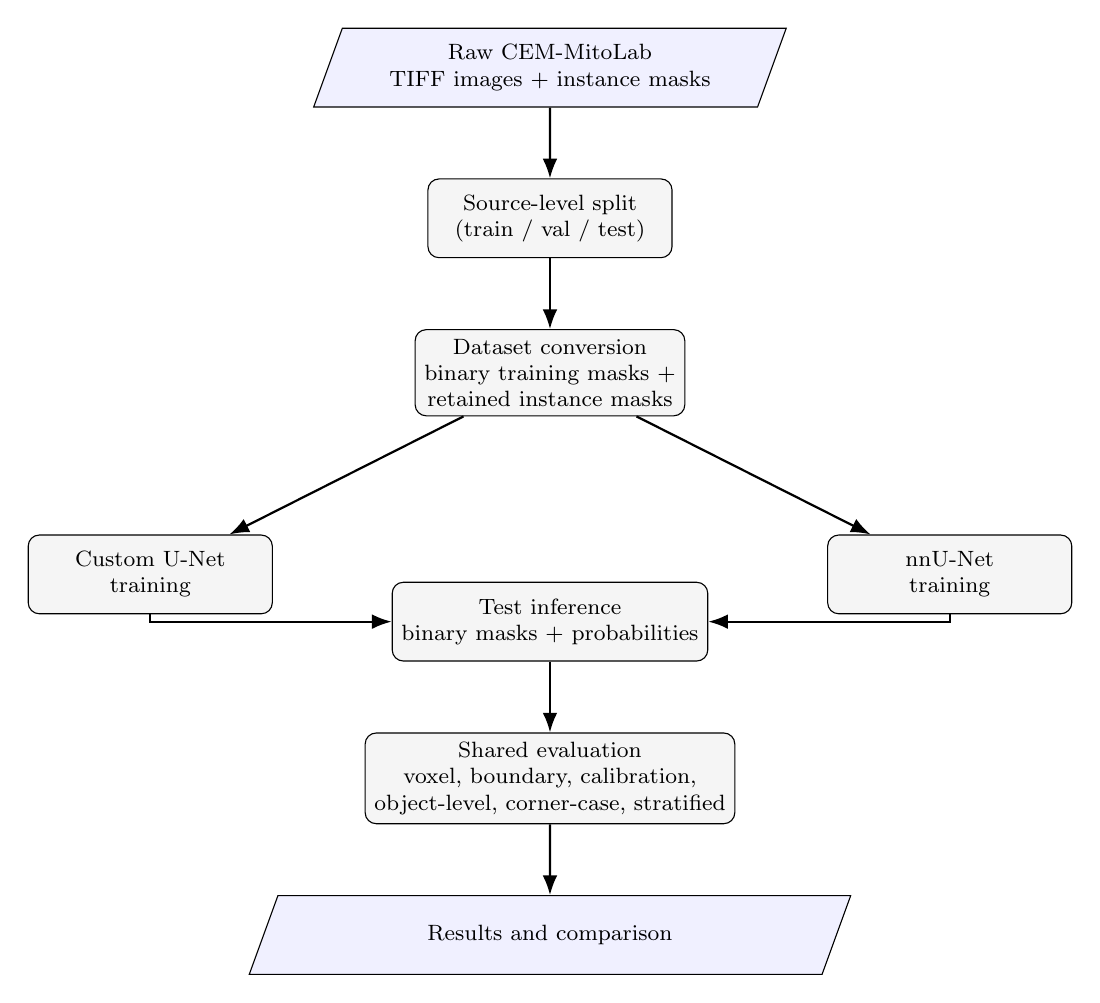
\begin{tikzpicture}[
    node distance=9mm and 12mm,
    every node/.style={font=\footnotesize, align=center},
    box/.style={draw, rounded corners, minimum width=31mm, minimum height=10mm, fill=gray!8},
    io/.style={draw, trapezium, trapezium left angle=70, trapezium right angle=110,
               minimum width=31mm, minimum height=10mm, fill=blue!6},
    decision/.style={draw, diamond, aspect=1.8, minimum width=24mm, minimum height=10mm, fill=green!6},
    arrow/.style={-{Latex[length=2.5mm]}, thick}
]
\node[io] (raw) {Raw CEM-MitoLab\\TIFF images + instance masks};
\node[box, below=of raw] (split) {Source-level split\\(train / val / test)};
\node[box, below=of split] (convert) {Dataset conversion\\binary training masks +\\retained instance masks};
\node[box, below left=15mm and 18mm of convert] (unet) {Custom U-Net\\training};
\node[box, below right=15mm and 18mm of convert] (nnunet) {nnU-Net\\training};
\node[box, below=21mm of convert] (infer) {Test inference\\binary masks + probabilities};
\node[box, below=of infer] (eval) {Shared evaluation\\voxel, boundary, calibration,\\object-level, corner-case, stratified};
\node[io, below=of eval] (results) {Results and comparison};

\draw[arrow] (raw) -- (split);
\draw[arrow] (split) -- (convert);
\draw[arrow] (convert) -- (unet);
\draw[arrow] (convert) -- (nnunet);
\draw[arrow] (unet) |- (infer);
\draw[arrow] (nnunet) |- (infer);
\draw[arrow] (infer) -- (eval);
\draw[arrow] (eval) -- (results);
\end{tikzpicture}
\caption{Overview of the experimental pipeline. The two
models share the same source-level split and rejoin for a common
evaluation stage.}
\label{fig:method-pipeline}
\end{figure}

\section{Dataset Description and Preprocessing}
\label{sec:impl-pipeline}

CEM-MitoLab consists of 2D electron microscopy slices with instance-labelled
mitochondria masks. For the present experiment, the raw images and annotations
were converted into a common format suitable for both model training and shared
evaluation. Binary semantic masks were derived from the instance labels for
training, while the original instance masks were retained for later
object-level evaluation.


Table~\ref{tab:split-summary} summarises the final split used throughout the
dissertation. Here, a \emph{biological source} refers to the source-level unit
from which multiple related slices may be drawn. All source assignment is
completed before slice counts are expanded, so no biological source contributes
images to more than one partition.

\begin{table}[H]
\centering
\small
\caption{Final source-level and slice-level split used for all experiments.}
\label{tab:split-summary}
\begin{tabular}{lrrl}
\toprule
\textbf{Partition} & \textbf{Sources} & \textbf{Slices} & \textbf{Role} \\
\midrule
Train      & 415 & 15{,}312 & Model fitting and augmentation \\
Validation & 89  & 3{,}247  & Model selection and early stopping \\
Test       & 89  & 3{,}312  & Final test set evaluation only \\
\bottomrule
\end{tabular}
\end{table}

The split was defined at the level of biological sources before being expanded
to slice counts, so no source contributes images to more than one partition.
The same split definition was used consistently for both models throughout
training, validation, and final testing. During training and validation, both
models used the same preprocessed inputs. For final inference, both were
applied to the same unseen raw test images before entering the shared
evaluation pipeline.

Because the slices vary in spatial dimensions, the preprocessing and batching
pipeline preserves the full field of view while adjusting inputs as needed to
remain compatible with the networks. This allows both training and inference to
proceed without cropping away biologically relevant image content.

\section{Model Configurations}

\subsection{Custom U-Net}

The custom model is a 2D U-Net implemented in PyTorch from scratch. It follows
the standard encoder-decoder design with skip connections, using four
down-sampling blocks and a bottleneck, with channel widths 64, 128, 256, 512,
and 1024 before the decoder upsamples back to full resolution. Each
convolutional block applies two 3$\times$3 convolutions followed by instance
normalisation and rectified linear unit (ReLU) activations
\citep{nair2010relu}. Instance normalisation was chosen because the custom
model trains with a batch size of 4, for which batch-normalisation statistics
are unstable.

To make the comparison closer to nnU-Net, the U-Net now predicts two classes
(background and mitochondria) and is trained with a combined cross-entropy plus
soft Dice objective. For a training set of $N$ pixels, with class probability
$p_{i,c}$ and target label $y_{i,c}$ for pixel $i$ and class $c$, the
cross-entropy term is
\[
\mathcal{L}_{\mathrm{CE}} = - \frac{1}{N} \sum_{i=1}^{N} \sum_{c} y_{i,c} \log p_{i,c}.
\]
For the foreground class alone, the soft Dice loss is
\[
\mathcal{L}_{\mathrm{Dice}} =
1 - \frac{2 \sum_{i=1}^{N} p_i y_i + \varepsilon}
{\sum_{i=1}^{N} p_i + \sum_{i=1}^{N} y_i + \varepsilon},
\]
where $p_i$ and $y_i$ denote the predicted foreground probability and the
binary foreground label, respectively. The total training objective is
\[
\mathcal{L} = \mathcal{L}_{\mathrm{CE}} + \mathcal{L}_{\mathrm{Dice}}.
\]
This combined objective follows the standard nnU-Net formulation and the common
soft Dice approach used in biomedical segmentation \citep{isensee2021nnu,
milletari2016vnet}. The Dice term is applied only to the foreground class, so
the training setup remains close to that of nnU-Net. During training and validation, the reported
Dice is also aligned with nnU-Net: it is computed from epoch-level hard
true-positive, false-positive, and false-negative counts rather than as a mean
of per-image Dice values.

\subsection{nnU-Net}

nnU-Net was used in its standard form, without changing the way it trains. For
this dataset it selected the 2D configuration, with a
patch size of 512$\times$512 and batch size 12. The resulting network is a
plain convolutional U-Net with eight stages, feature widths
\{32, 64, 128, 256, 512, 512, 512, 512\}, instance normalisation, and leaky
rectified linear unit (LeakyReLU) activations \citep{maas2013rectifier}. These choices come directly from nnU-Net's
planning stage and define the external baseline used in the comparison.

Table~\ref{tab:model-summary} summarises the main design and training
differences between the two systems.

\begin{table}[H]
\centering
\small
\caption{Summary of the two model setups used in the comparison.}
\label{tab:model-summary}
\renewcommand{\arraystretch}{1.15}
\setlength{\tabcolsep}{5pt}
\begin{tabularx}{\linewidth}{
>{\raggedright\arraybackslash}p{0.22\linewidth}
>{\raggedright\arraybackslash}X
>{\raggedright\arraybackslash}X}
\toprule
\textbf{Feature} & \textbf{Custom U-Net} & \textbf{nnU-Net} \\
\midrule
Task
& 2D semantic segmentation
& 2D semantic segmentation \\
Train/val input
& Same preprocessed training and validation images
& Same preprocessed training and validation images \\
Architecture
& Four-level U-Net with skip connections
& Automatically configured 2D convolutional U-Net \\
Channels/stages
& 64, 128, 256, 512, 1024
& 32, 64, 128, 256, 512, 512, 512, 512 \\
Normalisation
& Instance normalisation
& Instance normalisation \\
Activation
& Rectified linear unit activations
& Leaky rectified linear unit activations \\
Loss
& Combined cross-entropy and soft Dice objective
& Combined cross-entropy and Dice objective \\
Batch size
& 4
& 12 \\
Probability export
& Binary masks and probability maps exported for shared evaluation
& Binary masks and probability maps exported for shared evaluation \\
\bottomrule
\end{tabularx}
\end{table}

\section{Training and Inference Procedure}

\subsection{Software and Compute Environment}

The custom pipeline was implemented in Python using PyTorch
\texttt{2.10.0+cu128}, with GPU execution through CUDA under SLURM. nnU-Net was used through its
v2.6 command-line interface as an external package rather than a modified code
fork. Both training pipelines were run as single-GPU jobs, primarily on an
NVIDIA GeForce RTX 2080 Ti (11\,GB VRAM), with 32\,GB RAM and two CPU workers.

\subsection{Training Procedure}

\subsubsection{U-Net}

The custom U-Net was trained with the AdamW optimiser
\citep{loshchilov2019decoupled} and an initial learning rate of $10^{-3}$.
Validation was performed every second epoch, and the learning rate was reduced
when validation performance stopped improving. Training was stopped early if
the validation loss failed to improve meaningfully over 50 validation checks.

Data augmentation was applied only to the training split. This consisted of
horizontal and vertical flips, 90-degree rotations, small brightness shifts,
contrast changes, and additive Gaussian noise. 

\subsubsection{nnU-Net}

nnU-Net was trained in its standard configuration for this dataset, using the
same fixed train and validation split as the custom U-Net. Validation-time
probability outputs were retained during training, and the final test-time
probability outputs were exported separately during inference for the later
calibration and threshold-sensitivity analyses. 

For both models, model selection was validation-based. During training, each
pipeline also tracked a Dice-style validation summary to monitor progress, but
this quantity was used only as a training signal and not as a final test-set
metric. In nnU-Net, the per-epoch validation log reports pseudo-Dice, while
checkpoint selection uses its exponential moving average (EMA pseudo-Dice)
\citep{isensee2021nnu}. For comparability, the custom U-Net also reports a
Dice-style validation summary based on epoch-level foreground counts rather
than a mean of per-image Dice scores.

\subsection{Model Prediction on the Test Set}

Prediction on the test set is run as a separate stage so that both models are
applied to the same unseen raw test images before entering the shared final
evaluation pipeline. For the custom U-Net, the best validation checkpoint is
applied to the 3,312 test cases. Then, the shared default threshold of 0.5 is used
to binarise the foreground probability map, and both binary masks and
compressed probability arrays are exported. U-Net test inference uses raw TIFF
images with z-score normalisation to match training as closely as possible.

For nnU-Net, the selected test-time checkpoint is applied to the same held-out
images, and both binary masks and probability maps are retained for the shared
evaluation stage. The final nnU-Net results therefore come from a single
trained fold rather than from predictions combined across multiple folds.

\section{Applied Evaluation Procedure}

The metric definitions and rationale are given in Chapter~3. This section
describes how that framework was operationalised in the present experiment. For
each test case, the shared evaluation procedure uses a binary prediction mask,
a foreground probability map, and the original instance-labelled ground truth.
The same post-processing and measurement steps are applied to both models.

\subsection{Case Grouping and Aggregation}

All evaluation is carried out on the same set of 3,312 test slices.
Because 618 of these are background-only, aggregate results are reported both
over the full test set and over the 2,694 GT-positive slices
that contain at least one mitochondrion in the ground truth. This distinction
is important because empty slices make some predictions easy and would
otherwise blur differences in foreground and object-level behaviour.

\subsection{Voxel-Level Metrics}

Voxel-level metrics are computed at foreground thresholds
\{0.3, 0.4, 0.5, 0.6, 0.7\}. At each threshold the evaluation records
foreground Dice, background Dice, mean Dice, IoU, precision, recall, HD95, and
boundary F1 at 2-pixel and 5-pixel tolerance. HD95 is computed from the distances 
between predicted and ground-truth boundary pixels, using Euclidean distance 
transforms, rather than from all pixels in the mask.
Expected Calibration Error (ECE) is computed from the probability maps using
15 bins. Threshold 0.5 is treated as the default operating point, and the
surrounding thresholds are used for the threshold-sensitivity analysis.

\subsection{Object-Level Metrics}

Predicted instances are recovered from each binary foreground mask by
connected-component labelling with a 3$\times$3 connectivity structure. In the
final reported analysis, all predicted components are retained before matching.
The predicted objects are then compared with the ground-truth instance masks by
building a full pairwise IoU matrix and applying Hungarian matching to obtain
one-to-one assignments \citep{kuhn1955hungarian, munkres1957algorithms}. This
produces absolute count error, signed count error, mean matched IoU
\citep{taha2015metrics}, Panoptic Quality at IoU $> 0.5$
\citep{kirillov2019panoptic}, object-level precision and recall at IoU
thresholds 0.3, 0.5, 0.7, and 0.9, and the merge, split, and connectivity
statistics. A predicted object overlapping multiple ground-truth mitochondria
is counted as a merge, whereas a ground-truth mitochondrion overlapped by
multiple predicted objects is counted as a split. A supplementary sensitivity
analysis in the appendix repeats the same evaluation with predicted components
smaller than 10 pixels removed before matching.

\subsection{High-Dice Corner Cases}

The evaluation also includes a rule-based corner-case diagnostic. A
\emph{high-Dice corner case} is defined as a test slice with
foreground Dice above 0.85 at the default threshold of 0.5, but with either
object count error greater than 4, merge rate greater than 0, or split rate
greater than 0. Reported corner-case rates are shown both across all high-Dice
test slices, which includes GT-empty cases, and across the GT-positive
high-Dice subset. All reported corner-case results use the no-filter object
metrics described above.

\subsection{Statistical Testing}

Direct model comparisons are performed on paired per-image results. The shared
case identifiers in the paired per-image result tables are aligned first, after
which each metric is tested with a two-sided Wilcoxon signed-rank test
\citep{wilcoxon1945individual}. Pairs containing \texttt{NaN} or infinite
values are removed on a per-metric basis so that each test is run only where
the relevant metric is defined for both models.

Formal inference is applied to the predefined set of 27 paired per-image
metrics described in Chapter~3, spanning voxel-level overlap, boundary,
calibration, threshold sensitivity, and object-level behaviour. Descriptive
quantities such as signed count error, raw merge and split event counts,
zero-Dice counts, missed-positive counts, GT-empty false positives, corner-case
rates, and stratified summaries are reported separately and are not included in
the multiple-testing procedure. Raw $p$-values are corrected using the
Benjamini--Hochberg false-discovery-rate procedure
\citep{benjamini1995controlling} with $\alpha = 0.05$.

\subsection{Stratified Analysis}

The main stratified analysis tests whether model differences change across image
conditions. GT-positive test slices are grouped by foreground
pixel-ratio quartile, where foreground ratio is the fraction of image pixels
labelled as mitochondria in the ground truth. The quartile boundaries are
computed once from the ground-truth distribution and then applied identically
to both models, so the grouping does not depend on model output. This produces
four strata of roughly equal size, each containing approximately 674
GT-positive test slices.

Within each stratum, the models are compared using the same key metrics as in
the main analysis, especially foreground Dice, split rate, object count error,
and Panoptic Quality.



\chapter{Results and Analysis}
\label{chap:results}

\section{Test-Set Overview}
\label{sec:test-overview}

This chapter presents the evidence used to answer the three research questions
posed in Chapter~1. First, it examines whether standard voxel-level metrics can
understate biologically meaningful differences between the models. Second, it
tests whether voxel-level summaries accurately reflect distinct biologically
relevant error patterns such as merges and splits. Third, it evaluates whether
predictions with strong voxel-level scores can still contain errors that would
matter in biological analysis.

The test set contains 3,312 images drawn from 89 biological sources not
seen during training. Of these, 2,694 (81.3\%) contain at least one
mitochondrion in the ground truth (\emph{GT-positive}), while the remaining 618
(18.7\%) are background-only slices. Because background-only images allow any
model to achieve trivially perfect background Dice and an object count of zero
by predicting nothing, the distinction between GT-positive and GT-empty cases is
maintained throughout the analysis. Unless otherwise stated, all aggregate
figures are reported over all 3,312 test images; supplementary GT-positive-only
figures are provided where the difference is meaningful.


\section{U-Net Evaluation}
\label{sec:unet-results}

\subsection{Training Convergence}
\label{sec:unet-convergence}

The custom U-Net was not trained for a fixed 1,000-epoch schedule. Validation is
performed every second epoch and training stops once validation loss fails to
improve for 50 validation checks. Under this rule the U-Net
stopped at epoch~186, with the best checkpoint selected at epoch~86 by
validation loss. The highest observed validation pseudo-Dice, a Dice-style
overlap summary computed on the validation set and used as a 
training-progress signal before final test-set evaluation, occurred slightly
later (0.817 at epoch~92). The checkpoint used for test inference remained the
best-loss model because the later gains in pseudo-Dice were not accompanied by
improved validation loss, as shown in Figure~\ref{fig:convergence}.

\begin{figure}[H]
\centering
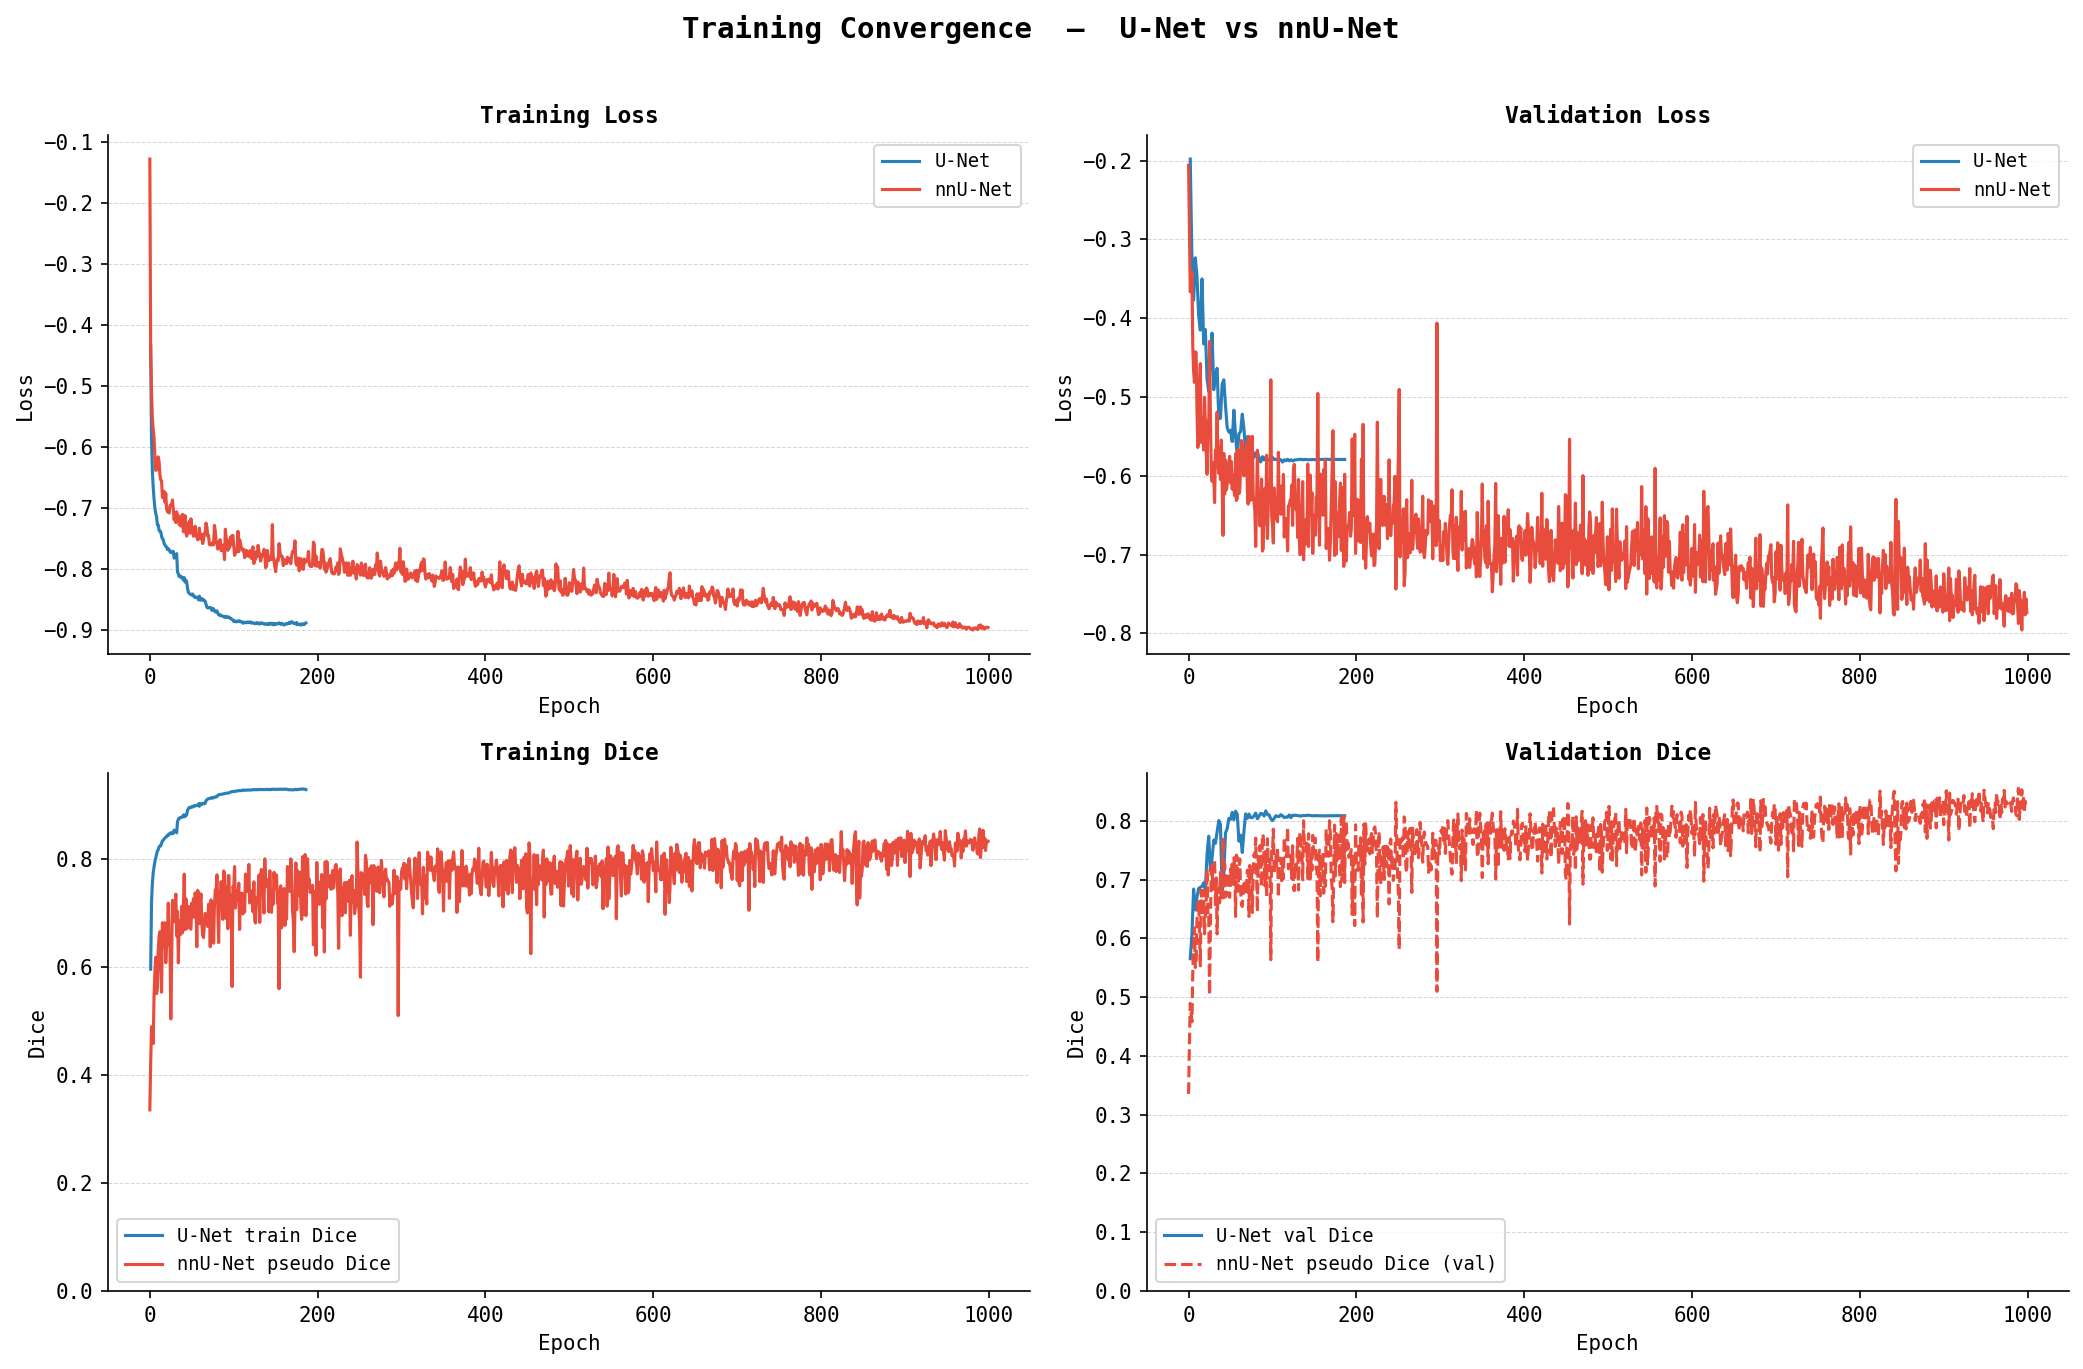
\includegraphics[width=\textwidth]{../figures/convergence/convergence.png}
\caption{Training convergence for the experiments. The custom U-Net
  early-stops at epoch~186, whereas nnU-Net completes the full 1,000-epoch
  schedule and continues to improve late in training.}
\label{fig:convergence}
\end{figure}

\subsection{Voxel-Level Performance}
\label{sec:unet-voxel}

Table~\ref{tab:unet-voxel} summarises the final U-Net voxel-level metrics at
the default threshold of 0.5.

\begin{table}[H]
\centering
\normalsize
\renewcommand{\arraystretch}{1.08}
\setlength{\tabcolsep}{3pt}
\caption{U-Net voxel-level metrics at threshold~0.5 on the test set.
  \emph{All}: all 3,312 cases; \emph{GT$+$}: GT-positive cases only
  (2,694 cases).}
\label{tab:unet-voxel}
\begin{tabular}{@{}lcccc@{}}
\toprule
 & \multicolumn{2}{c}{\textbf{All}}
 & \multicolumn{2}{c}{\textbf{GT$+$}} \\
\cmidrule(lr){2-3}\cmidrule(lr){4-5}
\textbf{Metric} & Mean $\pm$ SD & Median [IQR]
                & Mean $\pm$ SD & Median [IQR] \\
\midrule
Dice FG      & $0.636 \pm 0.357$ & $0.776\ [0.417{-}0.918]$
             & $0.612 \pm 0.331$ & $0.735\ [0.423{-}0.885]$ \\
Dice BG      & $0.985 \pm 0.024$ & $0.993\ [0.981{-}0.998]$
             & $0.983 \pm 0.025$ & $0.990\ [0.978{-}0.996]$ \\
Dice Mean    & $0.811 \pm 0.181$ & $0.878\ [0.693{-}0.954]$
             & $0.797 \pm 0.167$ & $0.858\ [0.696{-}0.936]$ \\
IoU (FG)     & $0.557 \pm 0.350$ & $0.633\ [0.264{-}0.849]$
             & $0.514 \pm 0.312$ & $0.582\ [0.269{-}0.794]$ \\
Precision    & $0.716 \pm 0.366$ & $0.899\ [0.607{-}0.969]$
             & $0.711 \pm 0.347$ & $0.885\ [0.614{-}0.941]$ \\
Recall       & $0.619 \pm 0.369$ & $0.750\ [0.325{-}0.949]$
             & $0.591 \pm 0.346$ & $0.686\ [0.328{-}0.899]$ \\
BF1 (2\,px)  & $0.626 \pm 0.355$ & $0.748\ [0.386{-}0.915]$
             & $0.599 \pm 0.328$ & $0.712\ [0.392{-}0.859]$ \\
BF1 (5\,px)  & $0.681 \pm 0.362$ & $0.839\ [0.491{-}0.973]$
             & $0.667 \pm 0.340$ & $0.804\ [0.496{-}0.929]$ \\
ECE          & $0.020 \pm 0.033$ & $0.009\ [0.002{-}0.025]$
             & $0.023 \pm 0.035$ & $0.013\ [0.005{-}0.028]$ \\
\bottomrule
\end{tabular}
\end{table}

At threshold~0.5, the U-Net mean
foreground Dice reaches 0.636 over the full test set and 0.612 over
GT-positive cases only, with mean IoU at 0.557. The medians are consistently
higher than the means. Most slices perform better than the average, but a
minority of hard cases pulls it down. Precision (0.716) exceeds recall (0.619),
which reflects a conservative foreground bias. Missed
foreground often corresponds to mitochondria that are only partially recovered,
or missed entirely.

\subsubsection{Hausdorff Distance}
HD95 is undefined on 438 images (13.2\%). Over the remaining 2,874 finite
cases, the mean HD95 is 47.2\,px and the median is 18.5\,px. These undefined
cases arise when either the prediction or the ground truth contains no
foreground boundary, so there is no valid pair of contours from which to
compute a Hausdorff distance. The gap between the mean and median indicates that
most predictions are much closer to the boundary than the mean alone suggests.
The mean is pulled upward by a smaller set of outliers with large contour
errors.

\subsubsection{Calibration}
The U-Net gives a
mean ECE of 0.020 and a median of 0.009, indicating that its foreground
probabilities are generally close to the observed fraction of foreground
pixels.

\subsection{Threshold Sensitivity}
\label{sec:unet-threshold}

Table~\ref{tab:unet-threshold} reports U-Net voxel metrics at five probability
thresholds spanning the range 0.30--0.70. All values are means over all 3,312
test cases; HD95 uses the per-threshold median to avoid inflation by the cases
that are undefined at each threshold.

\begin{table}[H]
\centering
\normalsize
\renewcommand{\arraystretch}{1.08}
\setlength{\tabcolsep}{4pt}
\caption{U-Net voxel metrics at five probability thresholds (mean over all
  3,312 test cases; HD95 is median of finite cases only).}
\label{tab:unet-threshold}
\begin{tabular}{@{}lrrrrr@{}}
\toprule
\textbf{Metric} & $t=0.30$ & $t=0.40$ & $t=0.50$ & $t=0.60$ & $t=0.70$ \\
\midrule
Dice FG      & 0.639 & 0.638 & 0.636 & 0.634 & 0.630 \\
Dice BG      & 0.985 & 0.985 & 0.985 & 0.985 & 0.985 \\
Dice Mean    & 0.812 & 0.812 & 0.811 & 0.810 & 0.808 \\
IoU (FG)     & 0.560 & 0.558 & 0.557 & 0.554 & 0.550 \\
Precision    & 0.702 & 0.710 & 0.716 & 0.721 & 0.726 \\
Recall       & 0.634 & 0.626 & 0.619 & 0.612 & 0.603 \\
BF1 (2\,px)  & 0.627 & 0.627 & 0.626 & 0.625 & 0.622 \\
BF1 (5\,px)  & 0.682 & 0.681 & 0.681 & 0.679 & 0.677 \\
HD95 (med.)  & 16.1  & 17.0  & 18.5  & 19.4  & 20.3  \\
\bottomrule
\end{tabular}
\end{table}

Foreground Dice varies by only 0.009 across thresholds 0.30--0.70 (from 0.639
to 0.630), with precision rising slightly and recall falling as the threshold
increases. The HD95 median also rises gradually from 16.1\,px to 20.3\,px
across the same range. Threshold choice is not a material source of variation
for the U-Net.

\subsection{Object-Level and Biological Performance}
\label{sec:unet-objects}

Table~\ref{tab:unet-objects} summarises the U-Net object-level metrics under
the connected-component recovery and Hungarian matching procedure.

\begin{table}[H]
\centering
\normalsize
\renewcommand{\arraystretch}{1.08}
\setlength{\tabcolsep}{3pt}
\caption{U-Net object-level metrics under the final no-filter connected-component
  analysis, with all predicted components retained before matching.
  \emph{All}: 3,312 test cases; \emph{GT$+$}: GT-positive cases only
  (2,694 cases).}
\label{tab:unet-objects}
\begin{tabular}{@{}lcccc@{}}
\toprule
 & \multicolumn{2}{c}{\textbf{All}} & \multicolumn{2}{c}{\textbf{GT$+$}} \\
\cmidrule(lr){2-3}\cmidrule(lr){4-5}
\textbf{Metric} & Mean $\pm$ SD & Median [IQR]
                & Mean $\pm$ SD & Median [IQR] \\
\midrule
GT objs/image       & $6.57 \pm 7.14$ & $3\ [1{-}11]$
                    & $8.08 \pm 7.11$ & $5\ [2{-}13]$ \\
Pred.\ objs/image   & $6.61 \pm 7.27$ & $4\ [1{-}11]$
                    & $7.89 \pm 7.35$ & $6\ [2{-}13]$ \\
Abs.\ count error   & $3.07 \pm 4.52$ & $2\ [0{-}4]$
                    & $3.54 \pm 4.68$ & $2\ [1{-}5]$ \\
Signed count error  & $0.04 \pm 5.46$ & $0\ [-2{-}1]$
                    & $-0.18 \pm 5.86$ & $0\ [-3{-}1]$ \\
Merge rate          & $0.041 \pm 0.099$ & $0.000$
                    & $0.050 \pm 0.108$ & $0.000\ [0.000{-}0.041]$ \\
Split rate          & $0.091 \pm 0.320$ & $0.000$
                    & $0.112 \pm 0.352$ & $0.000\ [0.000{-}0.091]$ \\
Conn.\ error        & $0.132 \pm 0.346$ & $0.000\ [0.000{-}0.151]$
                    & $0.162 \pm 0.378$ & $0.000\ [0.000{-}0.222]$ \\
Matched IoU         & $0.482 \pm 0.355$ & $0.625\ [0.000{-}0.788]$
                    & $0.592 \pm 0.299$ & $0.691\ [0.499{-}0.813]$ \\
PQ (IoU $>0.5$)     & $0.459 \pm 0.340$ & $0.445\ [0.170{-}0.715]$
                    & $0.395 \pm 0.275$ & $0.403\ [0.171{-}0.603]$ \\
\bottomrule
\end{tabular}
\end{table}

The object-level metrics present a more constrained view of performance than the
voxel-level summary. PQ reaches 0.459 over all test cases and 0.395 over
GT-positive cases only, while mean matched IoU is 0.482 over all cases. The 
near-zero signed count error is misleading, because missed objects and extra 
fragments partly cancel when averaged across slices.

\subsubsection{Object Count}
The average count error remains substantial at 3.07 over all test cases and 3.54
on GT-positive slices, with a median of 2 in both views. On GT-positive slices
the signed count error is still slightly negative ($-0.18$). The bias
is under-estimating the number of mitochondria present in
each slice, even though fragmented over-prediction elsewhere shifts the
overall mean closer to zero.

\subsubsection{Topology Errors}
The median merge and split rates are both zero, indicating that many images do
not exhibit topology errors. The mean split rate of 0.091 and connectivity
error of 0.132 show, however, that fragmentation remains concentrated in a
subset of difficult cases. Most images are unaffected, but the failures that do
occur are large enough to raise the mean.

\subsubsection{Object Precision and Recall}
Table~\ref{tab:unet-obj-pr} reports object-level precision and recall at four
IoU thresholds for all test cases.

\begin{table}[H]
\centering
\normalsize
\renewcommand{\arraystretch}{1.08}
\caption{U-Net object-level precision and recall at four IoU thresholds under
  the same no-filter connected-component analysis (mean $\pm$ SD over all
  3,312 test cases).}
\label{tab:unet-obj-pr}
\begin{tabular}{lcccc}
\toprule
\textbf{IoU thr.} & $\geq 0.3$ & $\geq 0.5$ & $\geq 0.7$ & $\geq 0.9$ \\
\midrule
Obj.\ Precision & $0.594 \pm 0.381$ & $0.557 \pm 0.382$ & $0.492 \pm 0.382$ & $0.247 \pm 0.366$ \\
Obj.\ Recall    & $0.593 \pm 0.374$ & $0.558 \pm 0.379$ & $0.494 \pm 0.384$ & $0.246 \pm 0.367$ \\
\bottomrule
\end{tabular}
\end{table}

At the lenient IoU threshold of 0.3, object-level precision reaches 0.594 and
recall 0.593. These fall to 0.557 and 0.558 at IoU 0.5 and then collapse to
0.247 and 0.246 at the strict threshold of 0.9. The model often places
mitochondria in roughly the right location. It is less reliable when considering
if those mitochondria were separated correctly.

\subsubsection{Failure Pattern}
The U-Net produces 551 zero-Dice slices, 278 completely missed GT-positive
slices, and 160 false-positive predictions on GT-empty slices. These counts
point to two recurring failure modes: complete misses on positive images and
false detections on background-only slices. The zero-Dice cases occur mainly
in slices with very small foreground extent, weak local contrast, or
fragmented predictions that fail to overlap the annotated mitochondria
sufficiently. The false positives on GT-empty slices show that fine
background texture or local noise is sometimes converted into small foreground
fragments when all predicted components are retained. In biological applications, 
these two errors have different consequences. Missed positive slices lead
to under-estimation of mitochondrial presence or density, whereas false
positives on empty slices inflate counts in regions that should contribute no
mitochondria at all. These failure modes therefore account for much of the
low-performing tail in the voxel-level distribution and help explain why the
mean is notably lower than the median. This interpretation is consistent with
the stratified analysis in Section~\ref{sec:stratified}, where the low-density
foreground quartile shows the weakest voxel-level and object-level results.

\section{nnU-Net Evaluation}
\label{sec:nnunet-results}

\subsection{Training Convergence}
\label{sec:nnunet-convergence}

nnU-Net trained for the full 1,000 epochs. The per-epoch validation
pseudo-Dice on the validation fold rose rapidly from 0.335 at epoch~0 to 0.746
by epoch~100, after which improvement continued more slowly, with a sustained
plateau through the middle training stage. A renewed improvement phase began
after epoch~800, reaching a peak per-epoch validation pseudo-Dice of 0.855 at
epoch~989 before declining slightly to 0.833 at the final epoch~999.
Checkpoint selection, however, used the EMA pseudo-Dice tracked by nnU-Net,
which also reached its best value at epoch~989 (0.830). The epoch~989
checkpoint was therefore used for test-set inference rather than the final
checkpoint from epoch~999. Figure~\ref{fig:convergence} compares the U-Net and
nnU-Net training traces directly.

\subsection{Voxel-Level Performance}
\label{sec:nnunet-voxel}

Table~\ref{tab:nnunet-voxel} summarises the voxel-level metrics at the default
prediction threshold of 0.5, for all test cases and for GT-positive cases only.
All values report mean $\pm$ standard deviation and the median with
interquartile range.

\begin{table}[H]
\centering
\normalsize
\renewcommand{\arraystretch}{1.08}
\setlength{\tabcolsep}{3pt}
\caption{nnU-Net voxel-level metrics at threshold~0.5 on the test set.
  \emph{All}: all 3,312 cases; \emph{GT$+$}: GT-positive cases only (2,694 cases).}
\label{tab:nnunet-voxel}
\begin{tabular}{@{}lcccc@{}}
\toprule
 & \multicolumn{2}{c}{\textbf{All}}
 & \multicolumn{2}{c}{\textbf{GT$+$}} \\
\cmidrule(lr){2-3}\cmidrule(lr){4-5}
\textbf{Metric} & Mean $\pm$ SD & Median [IQR]
                & Mean $\pm$ SD & Median [IQR] \\
\midrule
Dice FG      & $0.686 \pm 0.352$ & $0.854\ [0.520{-}0.943]$
             & $0.643 \pm 0.342$ & $0.804\ [0.441{-}0.909]$ \\
Dice BG      & $0.987 \pm 0.025$ & $0.995\ [0.986{-}0.999]$
             & $0.985 \pm 0.027$ & $0.993\ [0.984{-}0.997]$ \\
Dice Mean    & $0.837 \pm 0.179$ & $0.922\ [0.747{-}0.968]$
             & $0.814 \pm 0.174$ & $0.894\ [0.706{-}0.950]$ \\
IoU (FG)     & $0.614 \pm 0.350$ & $0.744\ [0.351{-}0.892]$
             & $0.554 \pm 0.326$ & $0.673\ [0.283{-}0.833]$ \\
Precision    & $0.773 \pm 0.350$ & $0.932\ [0.810{-}0.990]$
             & $0.750 \pm 0.350$ & $0.917\ [0.762{-}0.963]$ \\
Recall       & $0.659 \pm 0.365$ & $0.823\ [0.401{-}0.961]$
             & $0.610 \pm 0.354$ & $0.756\ [0.328{-}0.913]$ \\
BF1 (2\,px)  & $0.684 \pm 0.354$ & $0.837\ [0.516{-}0.967]$
             & $0.641 \pm 0.344$ & $0.775\ [0.435{-}0.909]$ \\
BF1 (5\,px)  & $0.729 \pm 0.354$ & $0.901\ [0.627{-}1.000]$
             & $0.696 \pm 0.350$ & $0.853\ [0.566{-}0.954]$ \\
ECE          & $0.018 \pm 0.038$ & $0.007\ [0.001{-}0.018]$
             & $0.022 \pm 0.040$ & $0.010\ [0.004{-}0.022]$ \\
\bottomrule
\end{tabular}
\end{table}

At threshold~0.5, nnU-Net reaches a mean foreground Dice of 0.686 over the full
test set and 0.643 over GT-positive cases only. As with the U-Net, the median
substantially exceeds the mean, so a minority of difficult images still drives
much of the remaining error. Precision again exceeds recall
(0.773 vs.\ 0.659). The model is still more prone to missing foreground than to
adding it, and that shows up later as object under-counting.

\subsubsection{Hausdorff Distance}
HD95 is undefined when either the prediction or the ground truth contains no
foreground, which affects 409 test images (12.3\%). Among the remaining 2,903
finite cases, the mean HD95 is 40.4\,px (SD~65.7), and the median is 8.9\,px.
This indicates that most predictions lie close to the ground-truth boundary,
with a smaller subset exhibiting large localised deviations. For GT-positive
cases only (2,363 finite), the mean rises to
49.6\,px and the median to 21.0\,px, as the easy background-only cases no
longer contribute.

\subsubsection{Calibration}
The mean ECE of 0.018 (median~0.007) indicates well-calibrated probability
maps overall. The low median relative to the mean
again reflects a small proportion of poorly calibrated images.

\subsection{Threshold Sensitivity}
\label{sec:nnunet-threshold}

\begin{table}[H]
\centering
\normalsize
\renewcommand{\arraystretch}{1.08}
\setlength{\tabcolsep}{4pt}
\caption{nnU-Net voxel metrics at five probability thresholds (mean over all
  3,312 test cases; HD95 is median of finite cases only).}
\label{tab:nnunet-threshold}
\begin{tabular}{@{}lrrrrr@{}}
\toprule
\textbf{Metric} & $t=0.30$ & $t=0.40$ & $t=0.50$ & $t=0.60$ & $t=0.70$ \\
\midrule
Dice FG      & 0.693 & 0.689 & 0.686 & 0.681 & 0.675 \\
Dice BG      & 0.988 & 0.988 & 0.987 & 0.987 & 0.987 \\
Dice Mean    & 0.840 & 0.838 & 0.837 & 0.834 & 0.831 \\
IoU (FG)     & 0.621 & 0.617 & 0.614 & 0.609 & 0.603 \\
Precision    & 0.764 & 0.768 & 0.773 & 0.776 & 0.779 \\
Recall       & 0.675 & 0.666 & 0.659 & 0.650 & 0.640 \\
BF1 (2\,px)  & 0.690 & 0.687 & 0.684 & 0.680 & 0.675 \\
BF1 (5\,px)  & 0.734 & 0.731 & 0.729 & 0.725 & 0.720 \\
HD95 (med.)  & 9.0   & 9.0   & 8.9   & 9.1   & 10.0  \\
\bottomrule
\end{tabular}
\end{table}

Foreground Dice varies by only 0.018 across thresholds 0.30--0.70 (from 0.693
to 0.675), and HD95 is essentially stable across this range. Threshold choice
is therefore not a major source of variation for nnU-Net.

\subsection{Object-Level and Biological Performance}
\label{sec:nnunet-objects}

Table~\ref{tab:nnunet-objects} summarises the object-level metrics under the
same no-filter connected-component recovery used for the U-Net. Ground-truth 
objects are taken from the original instance masks provided with the dataset, 
where background is labelled 0 and individual mitochondria are represented by 
nonzero integer labels.

\begin{table}[H]
\centering
\normalsize
\renewcommand{\arraystretch}{1.08}
\setlength{\tabcolsep}{3.0pt}
\caption{nnU-Net object-level metrics under the final no-filter
  connected-component analysis, with all predicted components retained before
  matching. \emph{All}: 3,312 test cases; \emph{GT$+$}: GT-positive cases only
  (2,694 cases).}
\label{tab:nnunet-objects}
\begin{tabular}{@{}lcccc@{}}
\toprule
 & \multicolumn{2}{c}{\textbf{All}} & \multicolumn{2}{c}{\textbf{GT$+$}} \\
\cmidrule(lr){2-3}\cmidrule(lr){4-5}
\textbf{Metric} & Mean $\pm$ SD & Median [IQR]
                & Mean $\pm$ SD & Median [IQR] \\
\midrule
GT objs/image        & $6.57 \pm 7.14$ & $3\ [1{-}11]$
                     & $8.08 \pm 7.11$ & $5\ [2{-}13]$ \\
Pred.\ objs/image    & $5.13 \pm 5.69$ & $3\ [0{-}9]$
                     & $6.23 \pm 5.72$ & $4\ [2{-}10]$ \\
Abs.\ count error    & $2.56 \pm 3.70$ & $1\ [0{-}3]$
                     & $3.07 \pm 3.86$ & $2\ [1{-}4]$ \\
Signed count error   & $-1.44 \pm 4.26$ & $0\ [-3{-}0]$
                     & $-1.85 \pm 4.57$ & $-1\ [-4{-}0]$ \\
Merge rate           & $0.035 \pm 0.090$ & $0.000$
                     & $0.044 \pm 0.098$ & $0.000$ \\
Split rate           & $0.041 \pm 0.266$ & $0.000$
                     & $0.050 \pm 0.294$ & $0.000$ \\
Conn.\ error         & $0.076 \pm 0.282$ & $0.000\ [0.000{-}0.053]$
                     & $0.093 \pm 0.310$ & $0.000\ [0.000{-}0.100]$ \\
Matched IoU          & $0.514 \pm 0.373$ & $0.698\ [0.000{-}0.826]$
                     & $0.632 \pm 0.310$ & $0.750\ [0.580{-}0.846]$ \\
PQ (IoU $>0.5$)      & $0.544 \pm 0.341$ & $0.577\ [0.299{-}0.831]$
                     & $0.468 \pm 0.295$ & $0.520\ [0.247{-}0.702]$ \\
\bottomrule
\end{tabular}
\end{table}



\subsubsection{Object Count}
The signed count error of $-1.44$ overall and $-1.85$ on GT-positive slices
confirms systematic under-prediction of objects. This is consistent with the
voxel-level recall gap (0.659 vs.\ precision 0.773): the model misses some
mitochondria even when it overlaps the foreground well at the pixel level.

\subsubsection{Topology Errors}
Merge rate (0.035) and split rate (0.041) have low mean values, and
the median for both is exactly zero, indicating that most images have no merge
or split events. Relative to the U-Net, both means are lower, especially for
split rate (0.041 vs.\ 0.091), so fragmentation is less frequent. The remaining
errors are still concentrated in a subset of difficult cases, rather than being
spread evenly across the test set.

\subsubsection{Object Precision and Recall}
Table~\ref{tab:nnunet-obj-pr} reports object-level precision and recall at four
IoU thresholds for all test cases.

\begin{table}[H]
\centering
\normalsize
\renewcommand{\arraystretch}{1.08}
\caption{nnU-Net object-level precision and recall at four IoU thresholds
  under the same no-filter connected-component analysis (mean $\pm$ SD over all
  3,312 test cases).}
\label{tab:nnunet-obj-pr}
\begin{tabular}{lcccc}
\toprule
\textbf{IoU thr.} & $\geq 0.3$ & $\geq 0.5$ & $\geq 0.7$ & $\geq 0.9$ \\
\midrule
Obj.\ Precision & $0.709 \pm 0.375$ & $0.676 \pm 0.377$ & $0.611 \pm 0.382$ & $0.329 \pm 0.390$ \\
Obj.\ Recall    & $0.633 \pm 0.367$ & $0.606 \pm 0.372$ & $0.556 \pm 0.378$ & $0.308 \pm 0.387$ \\
\bottomrule
\end{tabular}
\end{table}

At the lenient IoU threshold of 0.3, object-level precision reaches 0.709 and
recall 0.633. These fall to 0.676 and 0.606 at IoU 0.5 and decline further to
0.329 and 0.308 at the threshold of 0.9. Many mitochondria are detected at
the right location, but fewer are recovered with boundaries precise enough for
strict object-level agreement. PQ at IoU $>0.5$ (mean 0.544, median 0.577)
reflects both detection and localisation.

\subsubsection{Failure Pattern}
The nnU-Net produces 493 zero-Dice slices, 331 completely missed GT-positive
slices, and 78 false-positive predictions on GT-empty slices. As in the U-Net,
the zero-Dice cases occur mainly in difficult slices with very sparse
foreground, ambiguous local appearance, or predictions that remain close to
the mitochondria but do not overlap them sufficiently. The much lower
number of false positives on GT-empty slices indicates better suppression of
false foreground in purely background regions, although this failure mode is
not eliminated entirely. The
remaining missed-positive slices still produce under-counting of mitochondrial
presence, while the smaller GT-empty false-positive count reduces the risk of
inflated density estimates in empty regions. The same point appears in the
stratified analysis, where the low-density foreground quartile
gives the weakest overlap and object-level results. Relative to the U-Net,
nnU-Net also shows fewer GT-empty false positives (78 vs.\ 160) and fewer
zero-Dice slices overall (493 vs.\ 551).


\section{Model Comparison}
\label{sec:comparison}

The direct comparison shows that nnU-Net outperforms the U-Net on the standard voxel-level 
metrics, and that the gap becomes larger once object-level behaviour is considered.
nnU-Net leads in Dice, IoU, BF1, and finite HD95, while ECE differs only
slightly. Table~\ref{tab:model-comparison} summarises the key mean metrics at
threshold 0.5 and shows how the object-level analysis sharpens that ranking.

\begin{table}[!htbp]
\centering
\normalsize
\renewcommand{\arraystretch}{1.08}
\caption{Key mean metrics at threshold~0.5 on the test set. Difference is
  reported as nnU-Net minus U-Net.}
\label{tab:model-comparison}
\begin{tabular}{lrrr}
\toprule
\textbf{Metric} & \textbf{U-Net} & \textbf{nnU-Net} & \textbf{nn $-$ U} \\
\midrule
Foreground Dice         & 0.636 & 0.686 & +0.050 \\
IoU                     & 0.557 & 0.614 & +0.057 \\
Precision               & 0.716 & 0.773 & +0.057 \\
Recall                  & 0.619 & 0.659 & +0.040 \\
BF1 (2\,px)             & 0.626 & 0.684 & +0.058 \\
HD95 (paired finite mean, px)  & 43.06 & 39.78 & $-3.28$ \\
ECE                     & 0.020 & 0.018 & $-0.002$ \\
Count error signed      & $0.04$ & $-1.44$ & $-1.48$ \\
PQ (IoU $>0.5$)         & 0.459 & 0.544 & +0.084 \\
Obj.\ Precision @0.5    & 0.557 & 0.676 & +0.119 \\
Obj.\ Recall @0.5       & 0.558 & 0.606 & +0.048 \\
\bottomrule
\end{tabular}
\end{table}

The voxel-level gap is modest and consistent, whereas the object-level
separation is larger and more diagnostic, with a PQ advantage of 0.084 and an
object-precision advantage of 0.119 at IoU~0.5 for nnU-Net. Topology metrics
follow the same pattern: U-Net has both a
higher merge rate (0.041 vs.\ 0.035) and a much higher split rate (0.091 vs.\
0.041), also a larger connectivity error (0.132 vs.\ 0.076).

The same pattern is also visible at the distribution level, with the U-Net Dice
distribution shifted toward lower overlap (Appendix
Figure~\ref{fig:appendix-dice-overlay}).

\subsubsection{Trade-Offs}
U-Net misses fewer GT-positive slices (278 vs.\ 331) and its signed count
error is closer to zero overall, which might suggest comparable object
recovery. However, the near-zero signed count error
arises because extra fragments on difficult slices offset missed objects
elsewhere. Once the full object-level analysis is considered, U-Net has a
much higher split rate (0.091 vs.\ 0.041), a larger connectivity error
(0.132 vs.\ 0.076), more zero-Dice failures overall (551 vs.\ 493), fewer
very strong predictions with Dice $>0.9$ (1,005 vs.\ 1,295), and more
false positives on GT-empty slices (160 vs.\ 78). Fewer complete misses are
not enough to offset the weaker object separation and higher false-positive
rate.

Across the 27 paired metrics tested in the final evaluation, two-sided 
Wilcoxon signed-rank tests with Benjamini--Hochberg correction favour 
nnU-Net in all cases. This includes voxel overlap, boundary quality, 
calibration, and object-level metrics. These results provide strong paired
evidence within this test set, but because the tests are performed at slice
level rather than source level, they should be interpreted as support for
the observed comparison rather than as fully source-level inference.

\subsubsection{Practical Importance}
The Dice gap of 0.050 is relatively small when considered on its own. The object-level gaps are
larger: PQ differs by 0.084, object precision at IoU~0.5 by 0.119, and
split rate by more than a factor of two (0.091 vs.\ 0.041). These
differences reflect U-Net's stronger tendency to fragment individual
mitochondria into multiple predicted components. That would make object
counts, morphology summaries, and the separation of adjacent mitochondria
less reliable.

The advantage is also stable across threshold points. As shown in
Figure~\ref{fig:threshold-curves}, U-Net underperforms nnU-Net across the full
threshold range from 0.30 to 0.70, so the ranking does not depend on threshold
0.5 alone.

\begin{figure}[!htbp]
\centering
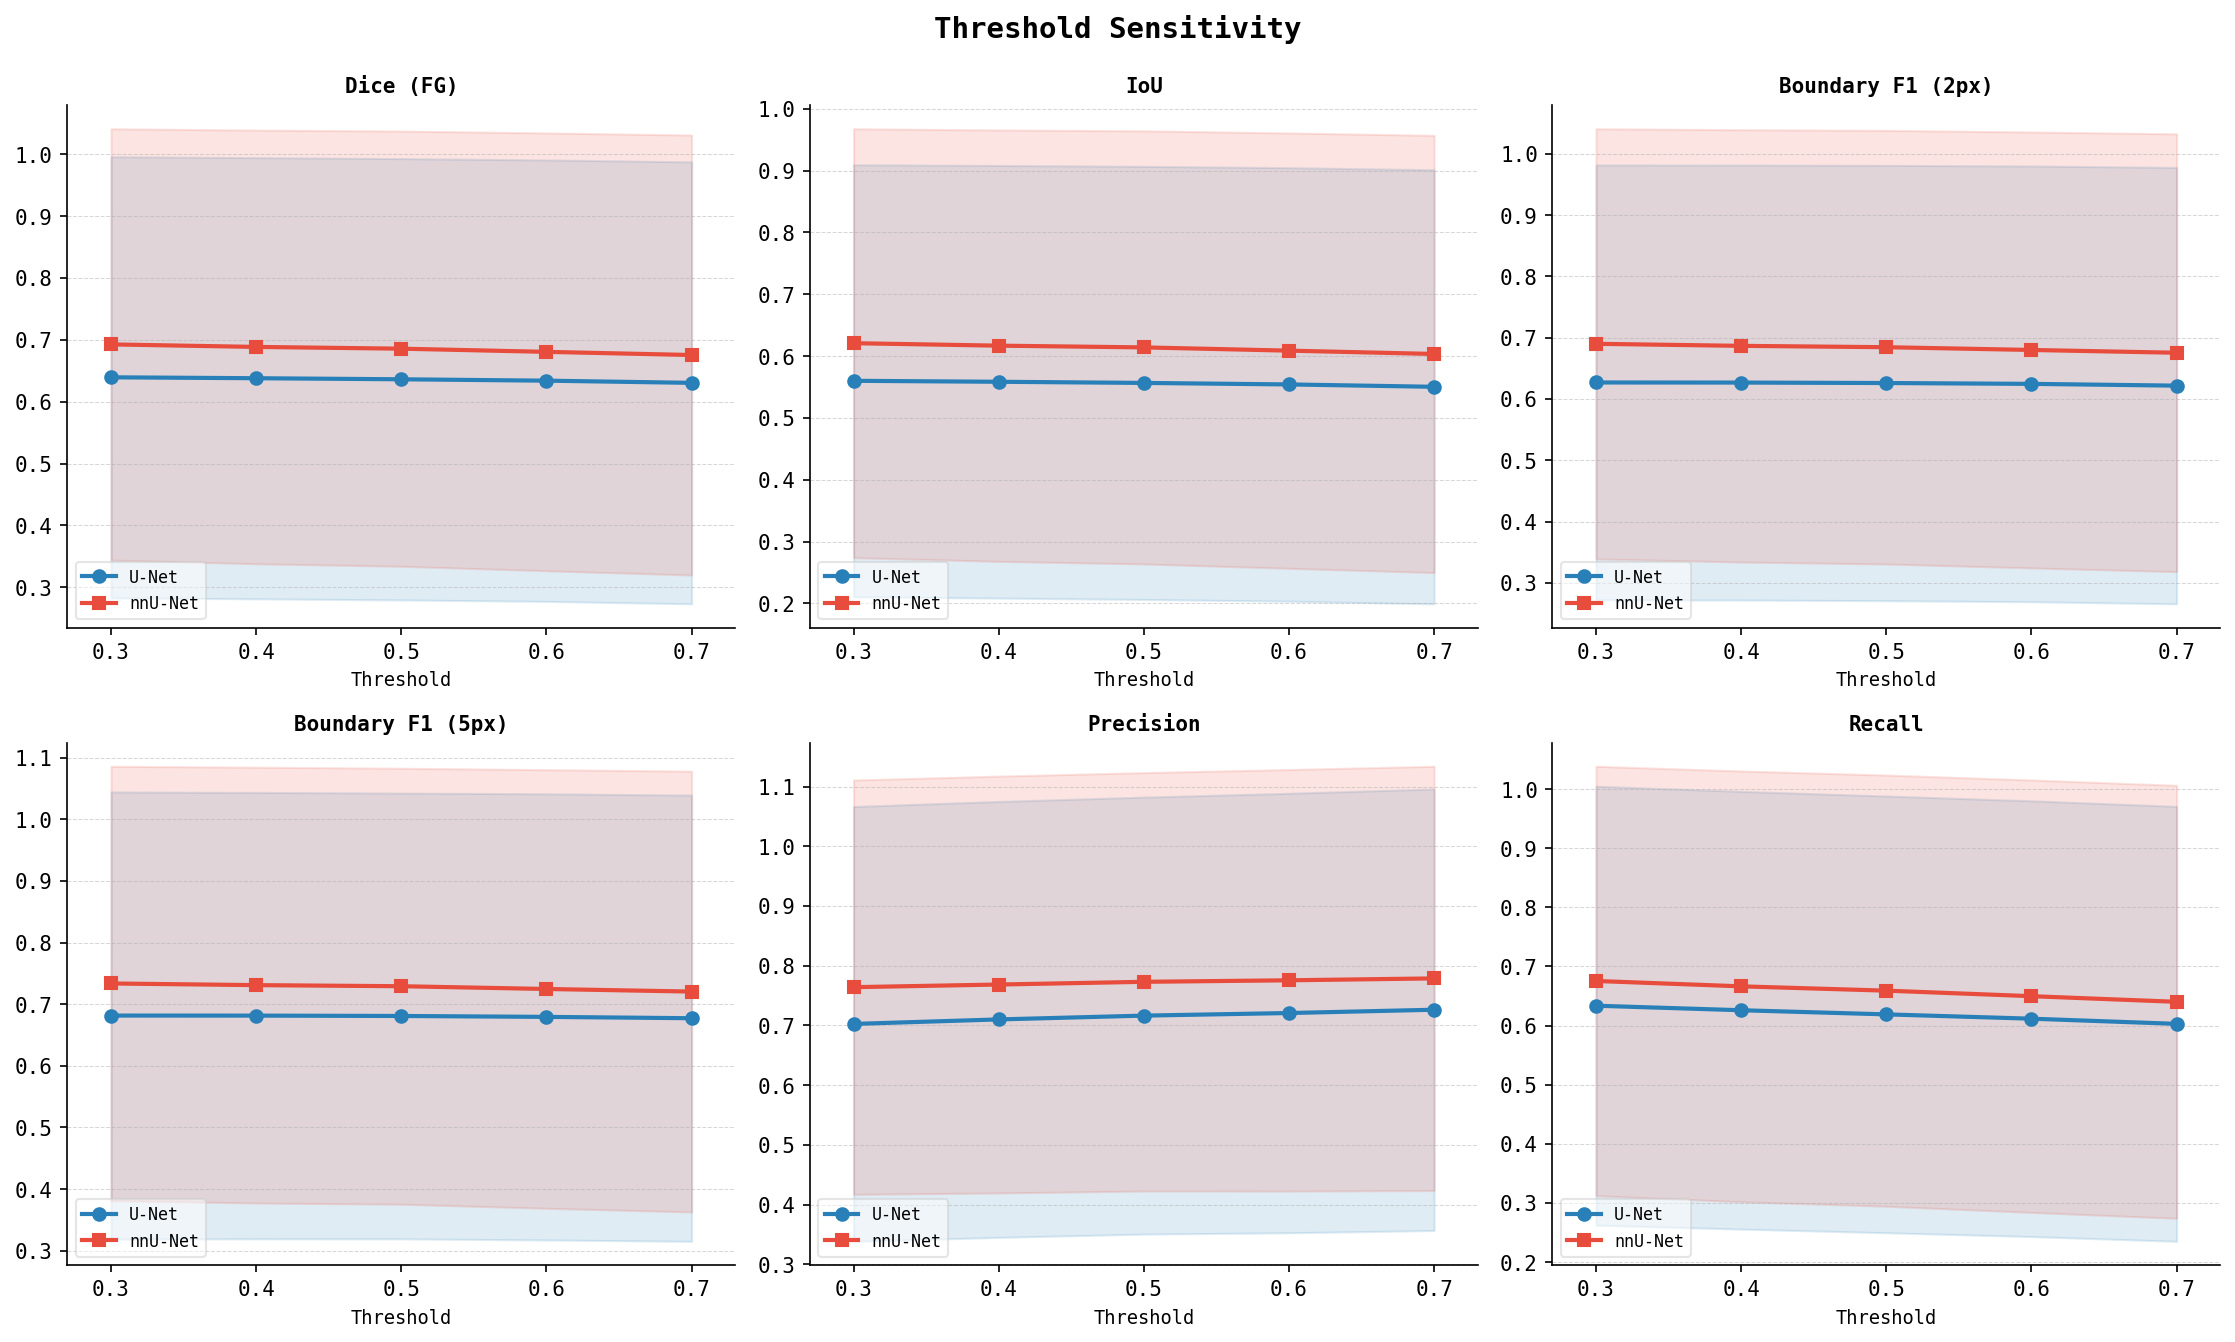
\includegraphics[width=\textwidth]{../figures/threshold_curves/threshold_sensitivity.png}
\caption{Threshold sensitivity curves for the test set. The ranking
  between U-Net and nnU-Net remains stable across the operating range
  0.30--0.70.}
\label{fig:threshold-curves}
\end{figure}

A supplementary Dice--PQ scatter is included in
Figure~\ref{fig:appendix-dice-vs-pq}. It shows the same pattern from another
angle: Dice and PQ are positively related for both models, and the spread
remains wide, especially in the high-Dice region.

\subsection{High-Dice Corner Cases}
This subsection addresses the third research question: whether a slice that
appears strong under voxel-level evaluation can still fail at the level of
individual mitochondria. The corner-case diagnostic uses Dice $>0.85$ as a
high-overlap threshold and then asks whether the same slice shows object count error
$>4$, merge rate $>0$, or split rate $>0$. Across all high-Dice slices, 373 of
1,340 U-Net cases (27.8\%) and 436 of 1,684 nnU-Net cases (25.9\%) still show
elevated object-level error. On the GT-positive high-Dice subset, the rates
rise to 373 of 882 U-Net cases (42.3\%) and 436 of 1,144 nnU-Net cases
(38.1\%).

If Dice $>0.85$ were used as a quality threshold, roughly one in four accepted
slices overall would still contain a biologically meaningful error. On
GT-positive accepted slices, the rate would be about two in five. These errors
include fragmented objects, merged clusters, count errors greater than four,
or combinations of these. Any downstream analysis that depends on object
count, morphology, or spatial separation would then inherit those errors.

Figure~\ref{fig:corner-case-examples} shows representative high-Dice failure modes directly. In the
U-Net example, the dense cluster is split into 12 predicted objects despite
Dice 0.953, with split rate 1.000. In the nnU-Net example,
most of the cluster is merged despite Dice 0.967, producing count error 14 and
merge rate 0.632. These are structural errors rather than minor boundary
deviations: one is driven by fragmentation and the other by merging. The
diagnostic uses Dice as the entry criterion, but the broader conclusion
concerns voxel-level sufficiency: strong voxel-level scores do not guarantee
reliable object recovery.

\begin{figure}[!htbp]
\centering
\begin{subfigure}[t]{0.98\textwidth}
  \centering
  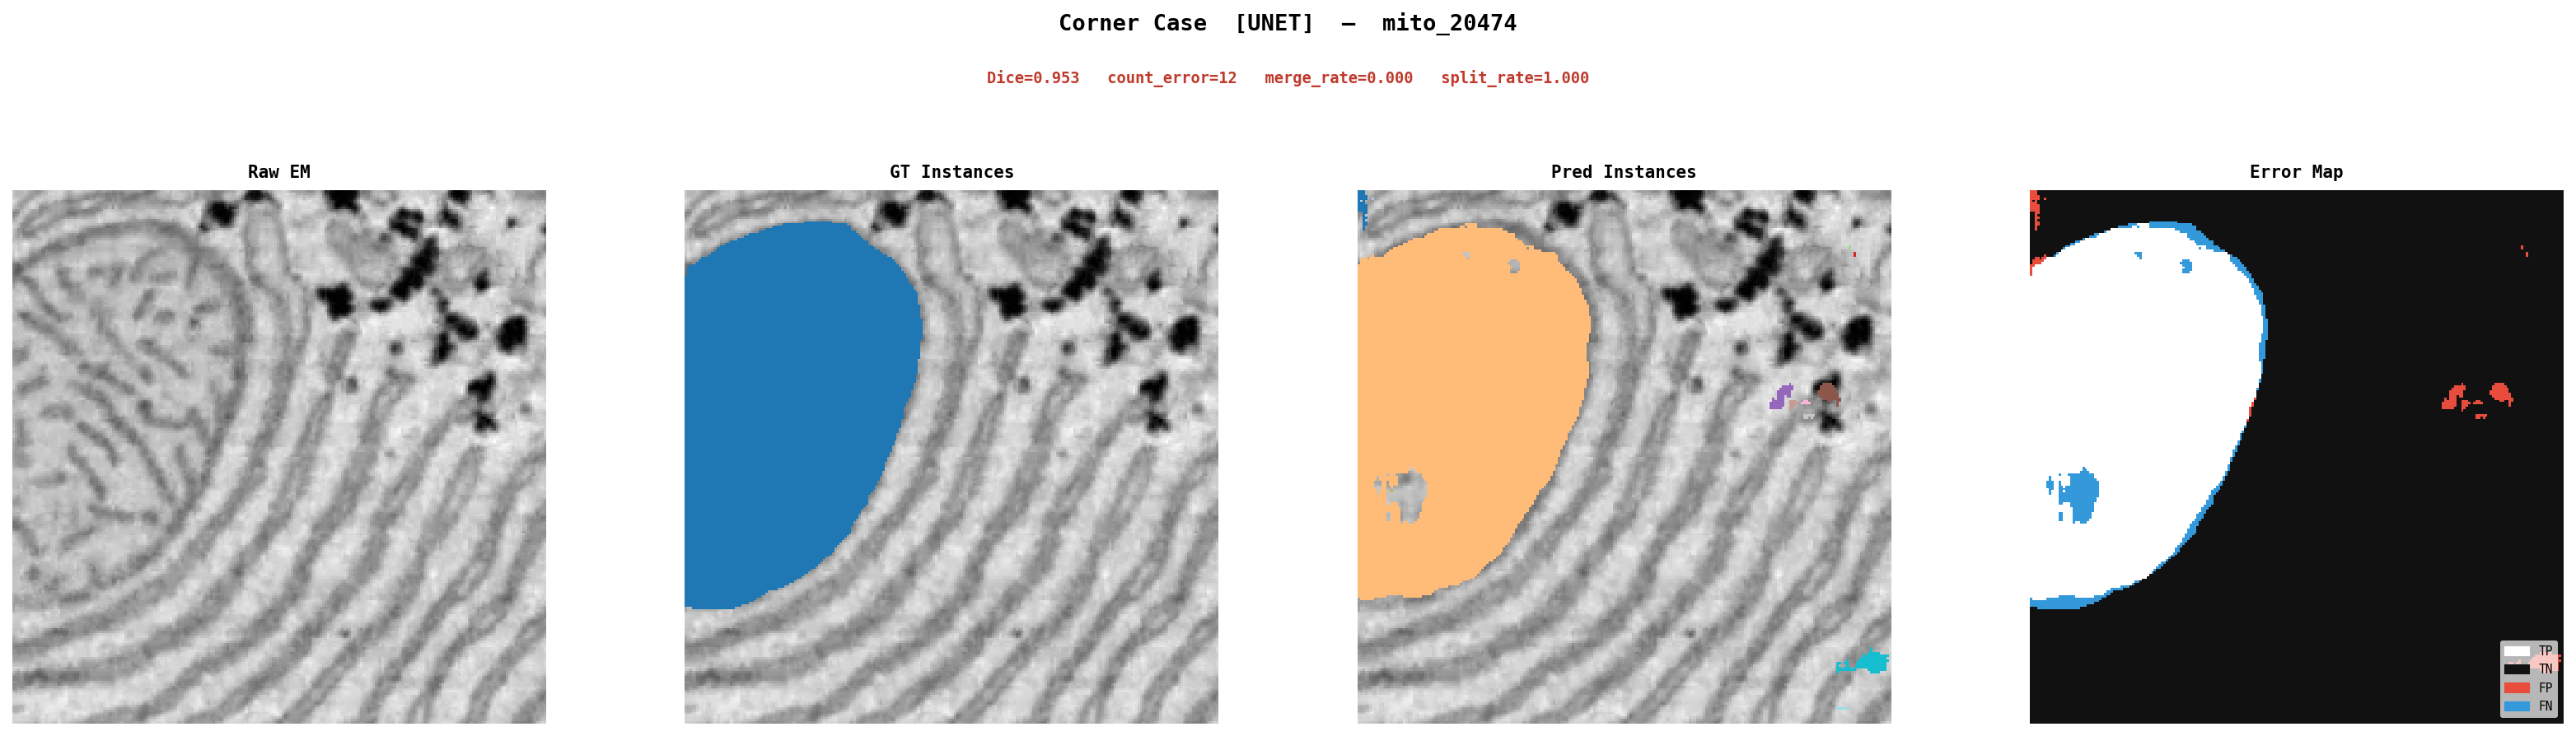
\includegraphics[width=\linewidth]{../figures/corner_cases/unet_mito_20474_corner_final.png}
  \caption{U-Net corner case: Dice 0.953, count error 12, split rate 1.000.}
\end{subfigure}

\vspace{0.8em}

\begin{subfigure}[t]{0.98\textwidth}
  \centering
  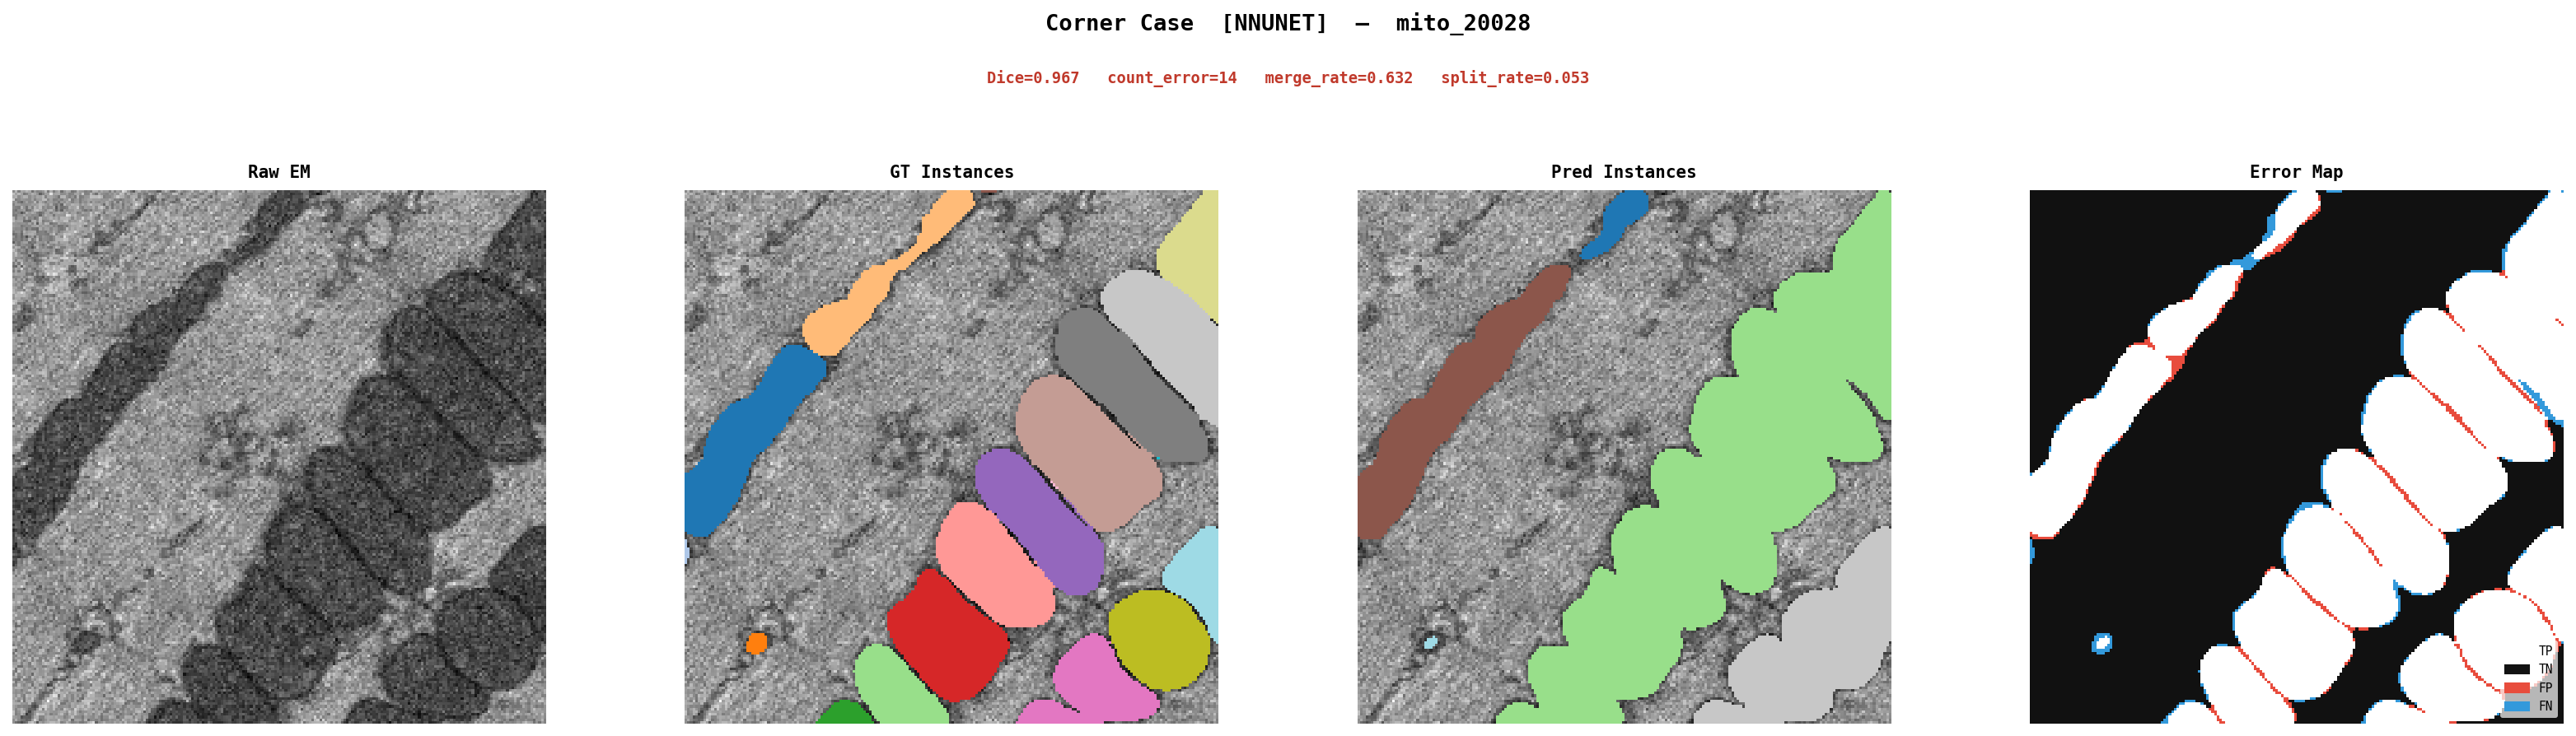
\includegraphics[width=\linewidth]{../figures/corner_cases/nnunet_mito_20028_corner_final.png}
  \caption{nnU-Net corner case: Dice 0.967, count error 14, merge rate 0.632.}
\end{subfigure}
\caption{Representative high-Dice corner cases from the test set. Both
  predictions score above 0.95 on Dice, yet both contain severe topology
  errors.}
\label{fig:corner-case-examples}
\end{figure}

Figure~\ref{fig:qualitative-comparison} shows two further examples where the
main difference is object separation rather than overall coverage. In example 1,
U-Net merges neighbouring mitochondria that nnU-Net keeps separate, despite
similar Dice, producing a PQ gap of 0.608 vs.\ 0.910. In example 2, U-Net draws
coarser boundaries in the denser region, reducing both Dice and PQ
(0.648/0.341 vs.\ 0.746/0.527). These examples make visible the mechanism
behind the aggregate PQ gap in Table~\ref{tab:model-comparison}: nnU-Net more
reliably separates adjacent mitochondria as distinct objects.

\begin{figure}[H]
\centering
\begin{subfigure}[t]{0.98\textwidth}
  \centering
  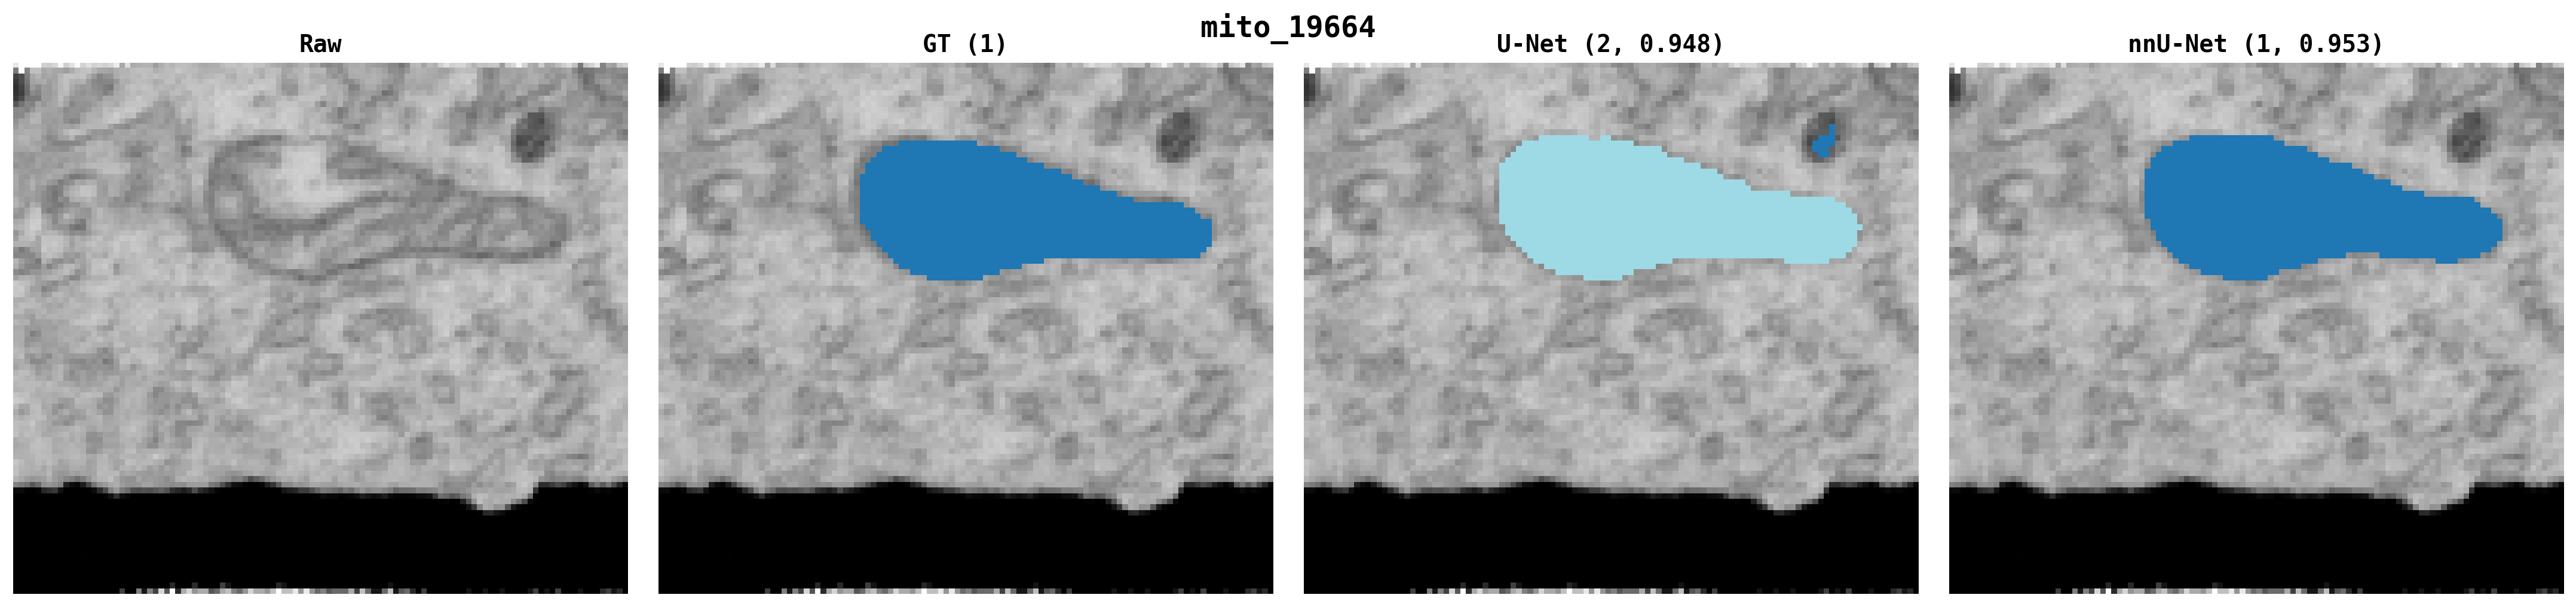
\includegraphics[width=\linewidth]{../figures/eval_instances/mito_19664_unet_vs_nnunet_instances.png}
  \caption{Qualitative example 1: similar Dice; PQ 0.608 vs.\ 0.910.}
\end{subfigure}

\vspace{0.8em}

\begin{subfigure}[t]{0.98\textwidth}
  \centering
  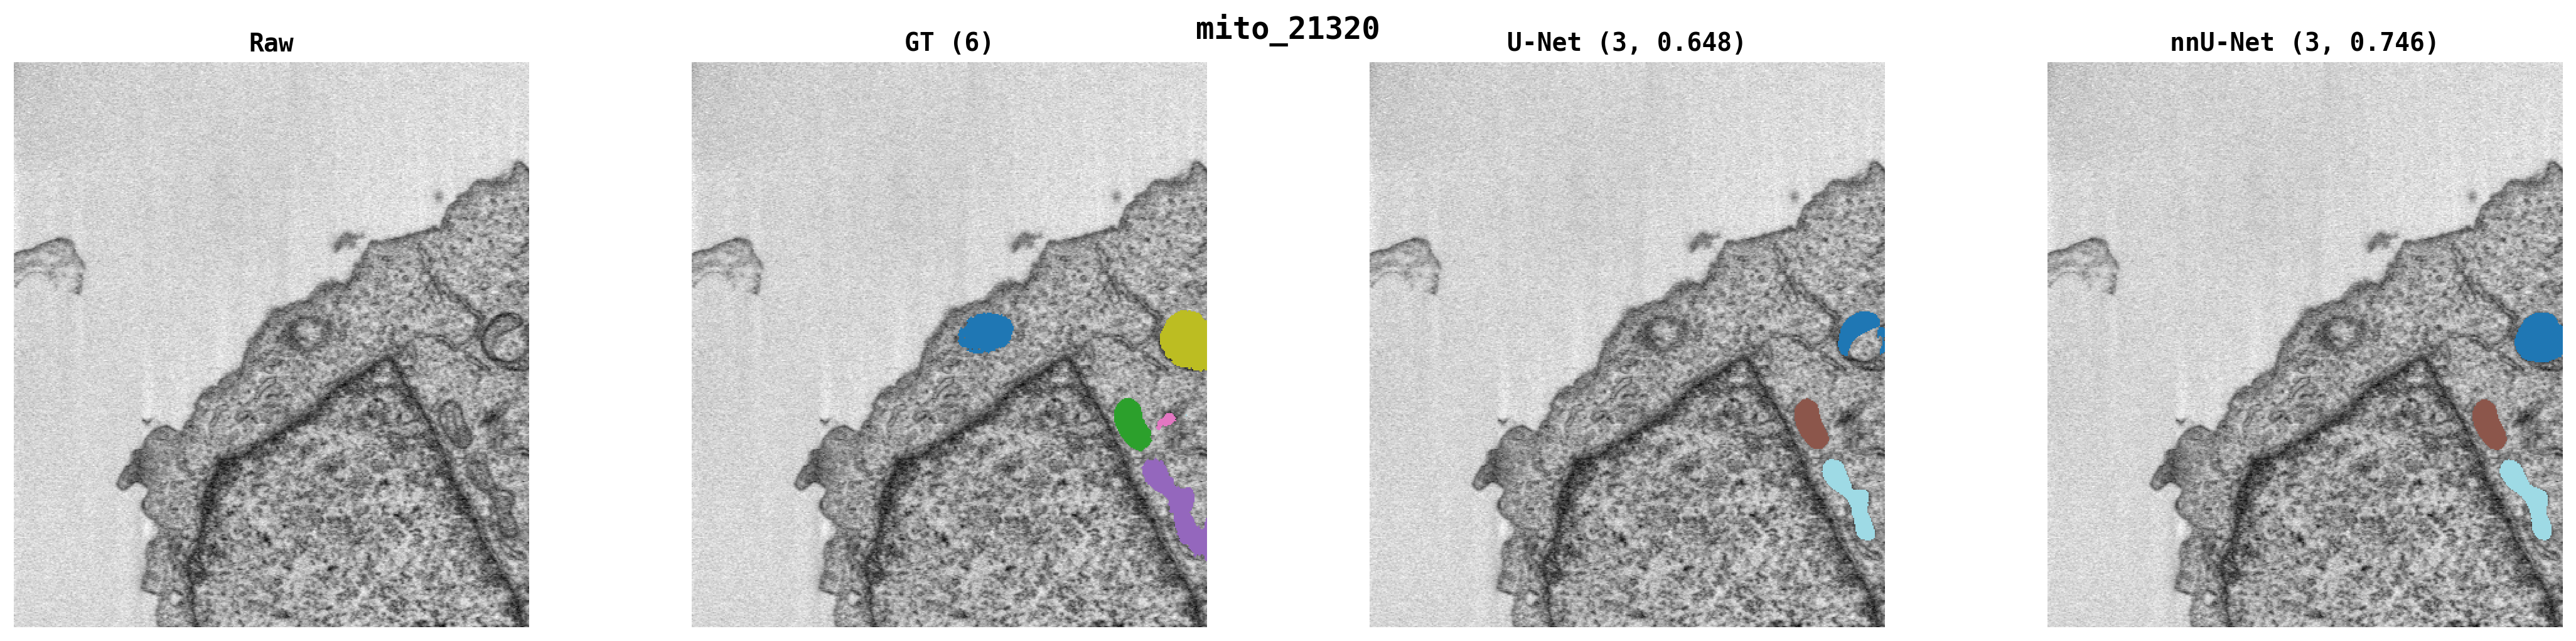
\includegraphics[width=\linewidth]{../figures/eval_instances/mito_21320_unet_vs_nnunet_instances.png}
  \caption{Qualitative example 2: denser slice; Dice/PQ 0.648/0.341 vs.\ 0.746/0.527.}
\end{subfigure}
\caption{Representative qualitative comparisons from the test set. In both
  examples nnU-Net preserves the separation of adjacent mitochondria more
  clearly.}
\label{fig:qualitative-comparison}
\end{figure}


\section{Stratified Analysis}
\label{sec:stratified}

Table~\ref{tab:fg-strat} stratifies GT-positive test images by foreground pixel
ratio quartile, with 674, 673, 673, and 674 images in Q1--Q4 respectively.
Foreground ratio is the fraction of image pixels labelled as mitochondria in
the ground truth. The quartile boundaries are derived from the GT-positive test
set: Q1 ($\leq 0.015$), Q2 (0.015--0.040), Q3 (0.040--0.102), and Q4
($>0.102$).

\begin{table}[H]
\centering
\normalsize
\renewcommand{\arraystretch}{1.08}
\setlength{\tabcolsep}{3pt}
\caption{Metrics stratified by foreground pixel-ratio quartile
  (GT-positive images only; $n \approx 674$ per quartile). The split-rate and
  PQ columns use the final no-filter connected-component analysis. `U'
  denotes U-Net and `nn' denotes nnU-Net.}
\label{tab:fg-strat}
\begin{tabular}{@{}lrrrrrr@{}}
\toprule
\textbf{Quartile} & \textbf{U Dice} & \textbf{nn Dice}
  & \textbf{U Split} & \textbf{nn Split}
  & \textbf{U PQ} & \textbf{nn PQ} \\
\midrule
Q1 ($\leq 0.015$)   & 0.398 & 0.435 & 0.039 & 0.020 & 0.290 & 0.325 \\
Q2 (0.015--0.040)   & 0.570 & 0.605 & 0.067 & 0.051 & 0.385 & 0.445 \\
Q3 (0.040--0.102)   & 0.722 & 0.767 & 0.109 & 0.046 & 0.486 & 0.591 \\
Q4 ($>$0.102)       & 0.759 & 0.763 & 0.231 & 0.083 & 0.419 & 0.510 \\
\bottomrule
\end{tabular}
\end{table}


Dice FG improves strongly with foreground density for both models, from 0.398
to 0.759 for U-Net and from 0.435 to 0.763 for nnU-Net. In the sparse first
quartile, the objects are small enough that even a few misplaced pixels can
reduce Dice. Performance then improves through Q2 and Q3 as the objects become
easier to localise and overlap.

Object-level quality follows a different pattern. PQ peaks in Q3 for both
models (0.486 for U-Net and 0.591 for nnU-Net) before falling in Q4, while
split rate rises sharply in the densest quartile, especially for U-Net (0.231
vs.\ 0.083). PQ falls in Q4 despite stronger Dice because dense packing
increases merges and splits, which PQ penalises directly but Dice can absorb
into its foreground-overlap score. At the voxel level, the Dice gap in Q4 is
small (0.759 vs.\ 0.763), which would make the models appear nearly equivalent 
if only overlap were considered. At the object level, the models remain clearly separated:
PQ stays higher for nnU-Net (0.510 vs.\ 0.419) and the split-rate gap widens
substantially in Q4.

\begin{figure}[H]
\centering
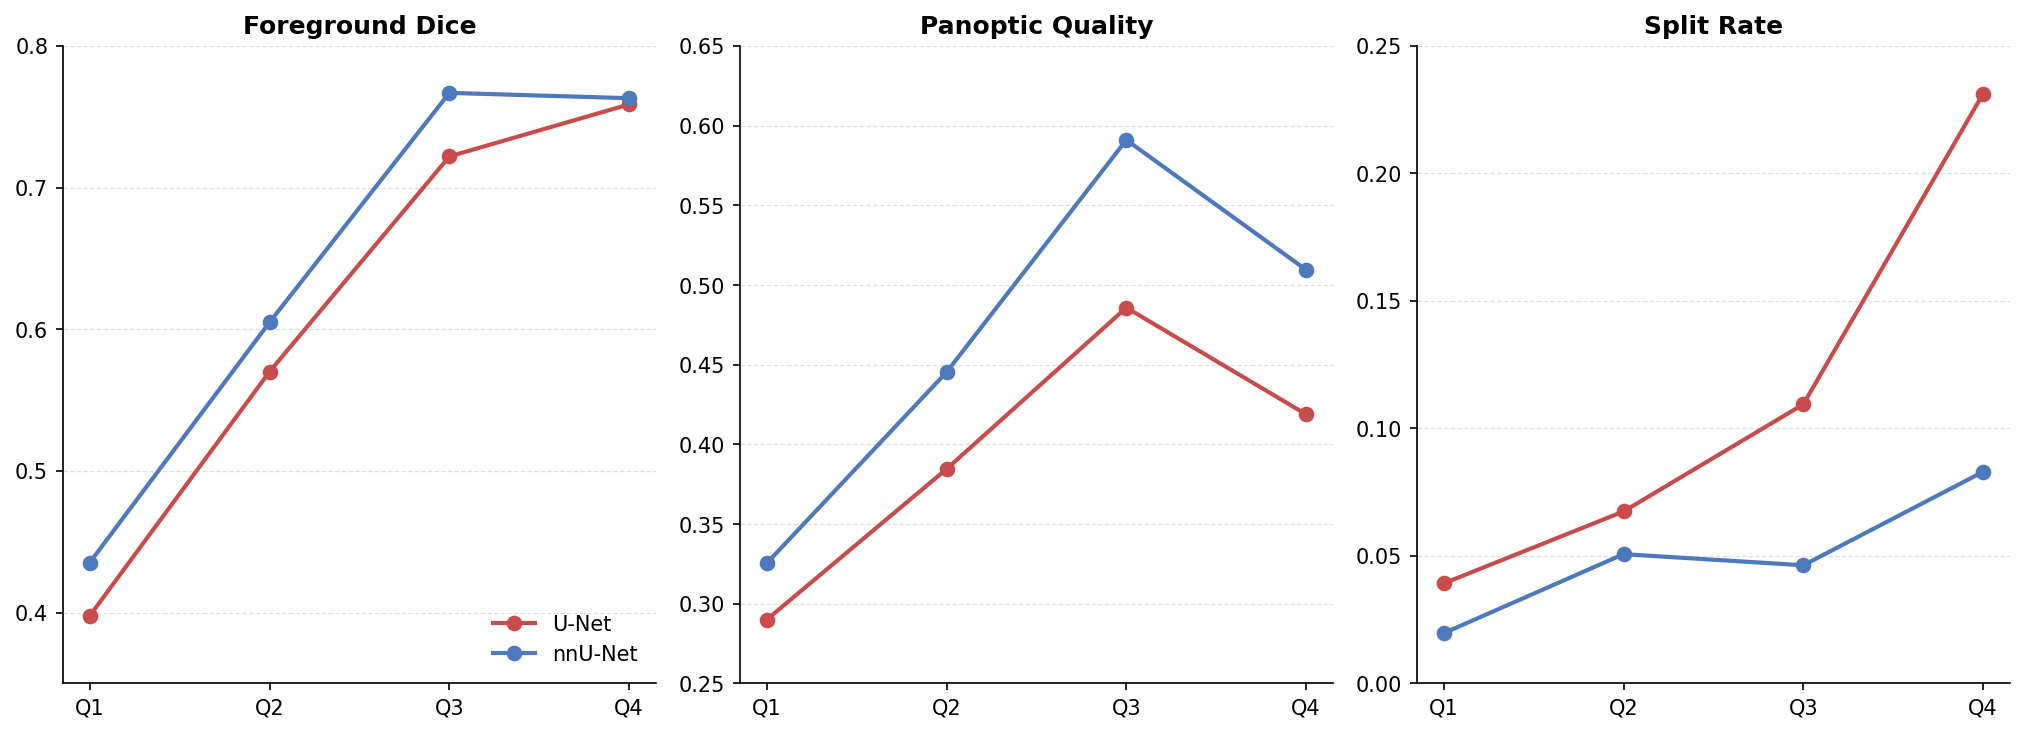
\includegraphics[width=\textwidth]{../figures/stratified/fg_density_quartiles.png}
\caption{Foreground-density stratification over GT-positive test slices. Dice
  improves with density for both models, but object-level quality peaks before
  the densest quartile and split rate rises sharply in Q4, especially for
  U-Net. The Dice curves converge in Q4 while the PQ and split-rate gaps widen.}
\label{fig:fg-density-stratified}
\end{figure}

Figure~\ref{fig:fg-density-stratified} shows this pattern. The Dice
curves draw closer in Q4, whereas split rate and PQ continue to separate the
models. A smaller voxel-level gap in dense images does not imply that the two
models perform equally well once individual mitochondria are evaluated at an
object-level. The dense-slice comparison shows the main result of the chapter most clearly:
voxel-level differences do not capture the object-level difference between the models. 



\chapter{Conclusions}
\section{Summary of Findings}
This chapter summarises the main findings and methodological conclusions.
Its structure follows the three research
questions posed in Chapter~1. These ask whether standard voxel-level metrics
can understate biologically meaningful differences between models, whether
they adequately reflect distinct error patterns such as merges and splits, and
whether strong voxel-level scores can still conceal errors that matter in
biological analysis.

\section{Main Conclusions}

\begin{enumerate}
  \item Standard voxel-level metrics can understate biologically meaningful
  differences between the models. nnU-Net is the stronger model overall, but
  the size of its advantage becomes clearer once the evaluation moves beyond
  voxel-level metrics alone. Foreground Dice differs by 0.050 (0.636 vs.\ 0.686),
  whereas PQ differs by 0.084 (0.459 vs.\ 0.544) and object precision at
  IoU~0.5 by 0.119 (0.557 vs.\ 0.676). In the densest quartile, the Dice gap
  almost disappears (0.759 vs.\ 0.763) while PQ and split rate remain clearly
  separated (0.419 vs.\ 0.510; 0.231 vs.\ 0.083).

  \item Standard voxel-level metrics do not adequately reflect distinct
  biologically relevant error patterns such as merges and splits. The direct
  comparison shows that U-Net has a higher merge rate (0.041 vs.\ 0.035),
  a much higher split rate (0.091 vs.\ 0.041), and a larger
  connectivity error (0.132 vs.\ 0.076). These differences matter because they
  change object counts and separation even when foreground overlap remains
  reasonably strong.

  \item Strong voxel-level scores can still conceal errors that matter in
  biological analysis. Under the Chapter~5 corner-case diagnostic, the
  corner-case rate is 27.8\% for U-Net and 25.9\% for nnU-Net across all
  high-scoring slices, rising to 42.3\% and 38.1\% on the GT-positive subset.
  Dice is used as the threshold in this diagnostic because it is the most
  common single overlap metric and the one most likely to be used on its own
  as a simple quality threshold. The qualitative corner-case examples show
  structural failures, including merged clusters and split objects, rather
  than minor boundary imprecision.
\end{enumerate}

In practice, this means an EM segmentation study in which individual mitochondria 
need to be counted and separated should not rely only on
voxel-level summaries. Dice, IoU, BF1, HD95,
and ECE remain useful, but they should be reported alongside boundary-aware and
object-level measures such as PQ, count error, and split or merge statistics
when downstream interpretation depends on individual mitochondria rather than
foreground overlap alone.

The central methodological contribution of this dissertation is a unified,
reproducible evaluation framework composed of four linked parts: a
standardised comparison pipeline, a biologically motivated metric set, a
rule-based corner-case diagnostic, and a stratified analysis of performance
across image conditions. Together, these make the metric gap measurable and
interpretable in a way that voxel-level evaluation alone does not.

\section{Limitations}
\label{sec:limitations}

\noindent\textbf{Model formulation.} Both models predict foreground as a
binary mask, and individual mitochondria are recovered afterward by
connected-component post-processing rather than learned directly during
training. The reported object-level results therefore should not be taken as
the best instance-level performance that more specialised end-to-end instance
segmentation models could achieve.

\noindent\textbf{Comparison setting.} nnU-Net is evaluated using a single fold
rather than its default five-fold ensemble, likely underestimating its full
capability. The U-Net was trained with batch size 4 due to GPU memory
constraints, compared to nnU-Net's batch size of 12, which may impede
convergence independently of architecture. The comparison is also confined to a
single dataset, so the results should not be assumed to generalise beyond the
conditions represented in CEM-MitoLab.

\noindent\textbf{Inferential scope.} Formal paired significance testing was
completed for the final evaluation using Wilcoxon signed-rank tests with
Benjamini--Hochberg correction, but the inferential analysis is still limited
to paired 2D slice-level metrics on a single dataset and therefore should not
be overgeneralised beyond this experimental setting.

\noindent\textbf{Rule-based corner-case diagnostic.} The corner-case analysis
is useful because it makes high-overlap failures easy to identify and inspect,
but it is based on a hand-specified rule (\emph{Dice}~$>0.85$ with a count
error greater than 4, a merge-rate trigger, or a split-rate trigger). Dice is
used here because it is the most common single overlap metric and the one most
likely to be treated as a standalone acceptance threshold. The reported rates
are therefore interpretable, but they depend on the chosen thresholds and on
whether they are summarised across all high-Dice slices or only the
GT-positive subset.

The main conclusion nevertheless remains clear. Within this controlled
comparison on CEM-MitoLab, voxel-level metrics were directionally useful but not
sufficient on their own, and the fuller metric set gave a more accurate picture 
of how useful the models are for biological analysis.

\section{Future Work}

\begin{enumerate}
  \item Evaluate nnU-Net with its full five-fold ensemble, to determine how much
  of the remaining performance gap reflects the single-fold restriction rather
  than the framework's intended inference setup.

  \item Compare the current semantic models against instance-aware
  alternatives, to test whether end-to-end instance modelling reduces the merge,
  split, and count errors highlighted in this dissertation.

  \item Apply the evaluation framework to additional EM datasets and model
  families, to determine which findings are specific to CEM-MitoLab and which
  transfer across imaging conditions and biological sources.

  \item Extend the corner-case analysis to 3D volumetric settings, where merge
  and split errors along the $z$-axis can become more consequential than in
  slice-wise 2D evaluation.
\end{enumerate}

% \bibliographystyle{plain}
\bibliographystyle{plainnat}
\bibliography{mybibfile}


% You may delete everything from \appendix up to \end{document} if you don't need it.
\appendix

\chapter{Supplementary Results}

This appendix collects supplementary statistical outputs, extended result
tables, and additional qualitative examples that support the main analysis in
Chapter~5.

\section{Full Paired Significance Tests}

Tables~\ref{tab:appendix-stats-voxel} and
\ref{tab:appendix-stats-object} report the full Wilcoxon signed-rank test
results with Benjamini--Hochberg-adjusted $p$-values for the final paired
evaluation. The difference column is reported as nnU-Net minus U-Net, so
positive values favour nnU-Net for higher-is-better metrics and negative values
favour nnU-Net for lower-is-better metrics.

\begin{table}[H]
\centering
\small
\caption{Supplementary paired significance tests for voxel-level, boundary, and
  calibration metrics.}
\label{tab:appendix-stats-voxel}
\begin{tabular}{lrrrr}
\toprule
\textbf{Metric} & \textbf{U-Net} & \textbf{nnU-Net} & \textbf{nn $-$ U} & \textbf{BH-adjusted $p$} \\
\midrule
Dice FG @0.5 & 0.636 & 0.686 & +0.049 & $8.55\times 10^{-50}$ \\
Dice BG @0.5 & 0.985 & 0.987 & +0.002 & $2.63\times 10^{-87}$ \\
IoU @0.5 & 0.557 & 0.614 & +0.057 & $1.93\times 10^{-57}$ \\
Precision @0.5 & 0.716 & 0.773 & +0.057 & $2.63\times 10^{-87}$ \\
Recall @0.5 & 0.619 & 0.659 & +0.040 & $4.57\times 10^{-21}$ \\
HD95 @0.5 & 43.060 & 39.783 & -3.277 & $1.97\times 10^{-11}$ \\
BF1 2px @0.5 & 0.626 & 0.684 & +0.058 & $1.02\times 10^{-62}$ \\
BF1 5px @0.5 & 0.681 & 0.729 & +0.048 & $9.16\times 10^{-40}$ \\
Dice FG @0.3 & 0.639 & 0.693 & +0.053 & $5.32\times 10^{-58}$ \\
Dice FG @0.4 & 0.638 & 0.689 & +0.051 & $1.59\times 10^{-53}$ \\
Dice FG @0.6 & 0.634 & 0.681 & +0.047 & $3.55\times 10^{-44}$ \\
Dice FG @0.7 & 0.630 & 0.675 & +0.045 & $5.00\times 10^{-40}$ \\
ECE & 0.020 & 0.018 & -0.002 & $1.85\times 10^{-46}$ \\
\bottomrule
\end{tabular}
\end{table}

\begin{table}[H]
\centering
\small
\caption{Supplementary paired significance tests for object-level metrics.}
\label{tab:appendix-stats-object}
\begin{tabular}{lrrrr}
\toprule
\textbf{Metric} & \textbf{U-Net} & \textbf{nnU-Net} & \textbf{nn $-$ U} & \textbf{BH-adjusted $p$} \\
\midrule
Abs count error & 3.066 & 2.559 & -0.507 & $1.73\times 10^{-12}$ \\
Merge rate & 0.041 & 0.035 & -0.006 & $3.15\times 10^{-8}$ \\
Split rate & 0.091 & 0.041 & -0.050 & $4.67\times 10^{-51}$ \\
Connectivity error & 0.132 & 0.076 & -0.056 & $3.59\times 10^{-57}$ \\
PQ @IoU 0.5 & 0.459 & 0.544 & +0.084 & $2.03\times 10^{-116}$ \\
Mean matched IoU & 0.482 & 0.514 & +0.032 & $5.52\times 10^{-60}$ \\
Obj.\ precision @0.3 & 0.594 & 0.709 & +0.115 & $3.36\times 10^{-106}$ \\
Obj.\ recall @0.3 & 0.593 & 0.633 & +0.039 & $2.43\times 10^{-19}$ \\
Obj.\ precision @0.5 & 0.557 & 0.676 & +0.119 & $1.50\times 10^{-109}$ \\
Obj.\ recall @0.5 & 0.558 & 0.606 & +0.047 & $1.69\times 10^{-30}$ \\
Obj.\ precision @0.7 & 0.492 & 0.611 & +0.119 & $1.92\times 10^{-114}$ \\
Obj.\ recall @0.7 & 0.494 & 0.556 & +0.061 & $9.18\times 10^{-52}$ \\
Obj.\ precision @0.9 & 0.247 & 0.329 & +0.082 & $3.43\times 10^{-95}$ \\
Obj.\ recall @0.9 & 0.246 & 0.308 & +0.062 & $4.03\times 10^{-68}$ \\
\bottomrule
\end{tabular}
\end{table}

\section{Sensitivity to Small-Object Filtering}

The earlier object-level evaluation removed predicted components smaller than
10 pixels before matching. Recomputing the full object-level analysis with all
predicted components retained did not change the ranking or the inferential
summary: nnU-Net still outperformed U-Net on all 27 paired metrics after
Benjamini--Hochberg correction. Retaining all predicted components did,
however, make fragmentation more visible, especially for the U-Net. Its split rate rose from
0.036 to 0.091 and its connectivity error from 0.077 to 0.132, whereas the
corresponding nnU-Net values rose from 0.023 to 0.041 and from 0.058 to
0.076. PQ decreased slightly for both models (U-Net 0.480 to 0.459; nnU-Net
0.551 to 0.544). The main conclusion is therefore robust, and retaining all
components is the more appropriate main analysis for this dissertation because
small recovered fragments are part of the failure mode under study.

\section{Extended Result Tables}

\subsection{GT-Empty Slice Behaviour}

Table~\ref{tab:appendix-gt-empty} isolates the 618 background-only test slices.
This makes the difference in empty-slice behaviour explicit: U-Net produces
false positives on 160 of 618 GT-empty slices (25.9\%), whereas nnU-Net does so
on 78 of 618 (12.6\%).
For overlap-style foreground metrics on GT-empty slices, an exactly empty
prediction is scored as perfect and any false-positive prediction is scored as
zero, which is why Dice FG, IoU, Precision, Recall, and BF1 collapse to the
same mean in this table.

\begin{table}[H]
\centering
\small
\caption{Supplementary results on GT-empty slices only at threshold~0.5.}
\label{tab:appendix-gt-empty}
\begin{tabular}{lrr}
\toprule
\textbf{Metric} & \textbf{U-Net} & \textbf{nnU-Net} \\
\midrule
Pred.\ foreground pixels (mean) & 329.654 & 111.466 \\
False-positive GT-empty slices & 160 / 618 & 78 / 618 \\
Dice FG (mean) & 0.741 & 0.874 \\
Dice BG (mean) & 0.997 & 0.999 \\
IoU (mean) & 0.741 & 0.874 \\
Precision (mean) & 0.741 & 0.874 \\
Recall (mean) & 0.741 & 0.874 \\
BF1 (2\,px) mean & 0.741 & 0.874 \\
BF1 (5\,px) mean & 0.741 & 0.874 \\
ECE (mean) & 0.005 & 0.002 \\
\bottomrule
\end{tabular}
\end{table}

\section{Supplementary Comparison Visuals}

Figure~\ref{fig:appendix-dice-overlay} gives the full foreground-Dice
distribution comparison, while Figure~\ref{fig:appendix-dice-vs-pq} shows the
corresponding Dice--PQ relationship over individual test slices.

\begin{figure}[H]
\centering
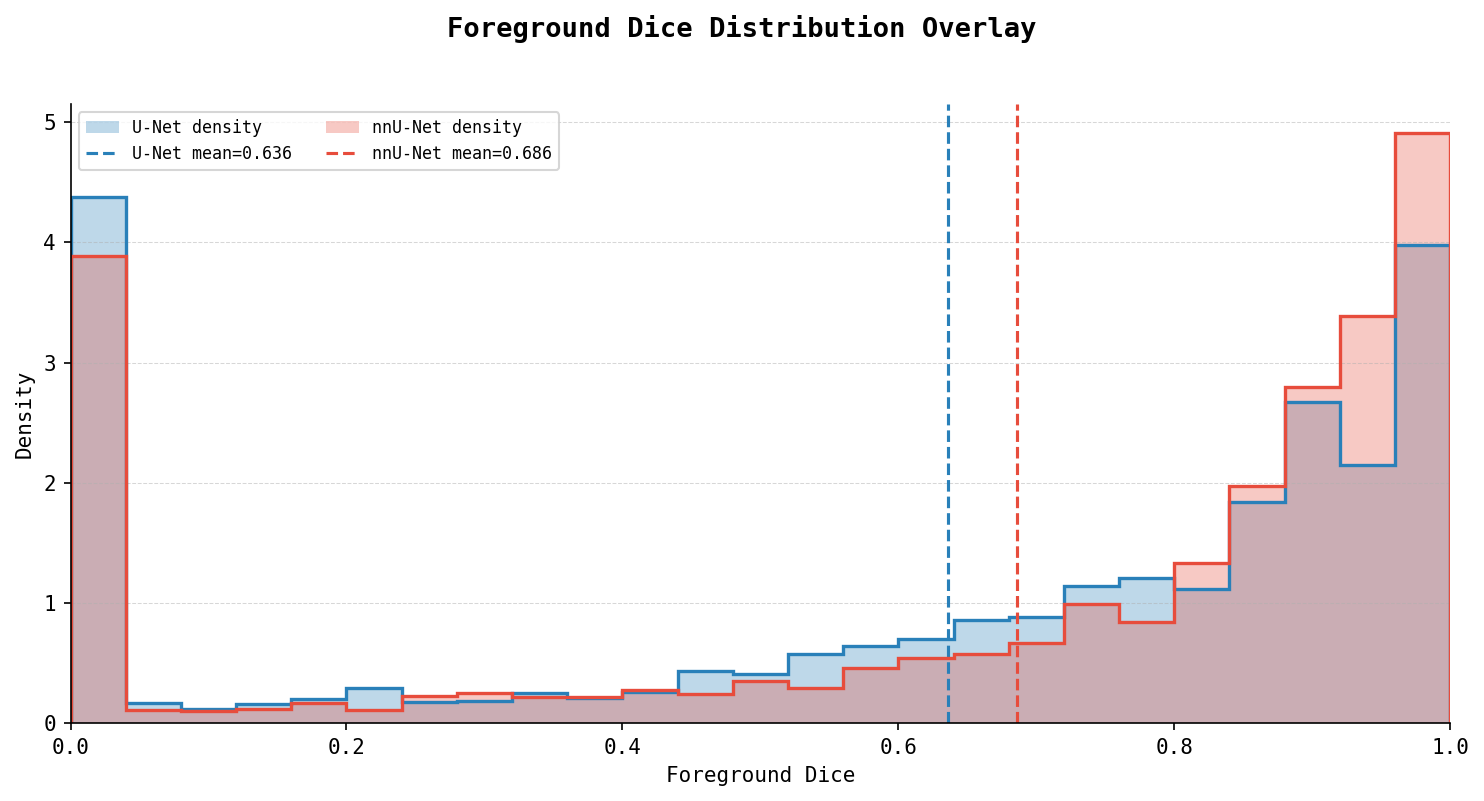
\includegraphics[width=0.92\textwidth]{../figures/dice_distribution_overlay.png}
\caption{Supplementary foreground Dice distributions for U-Net and nnU-Net over
  the test set. The U-Net distribution is shifted toward lower Dice,
  although both models retain a long left tail of difficult cases.}
\label{fig:appendix-dice-overlay}
\end{figure}

\begin{figure}[H]
\centering
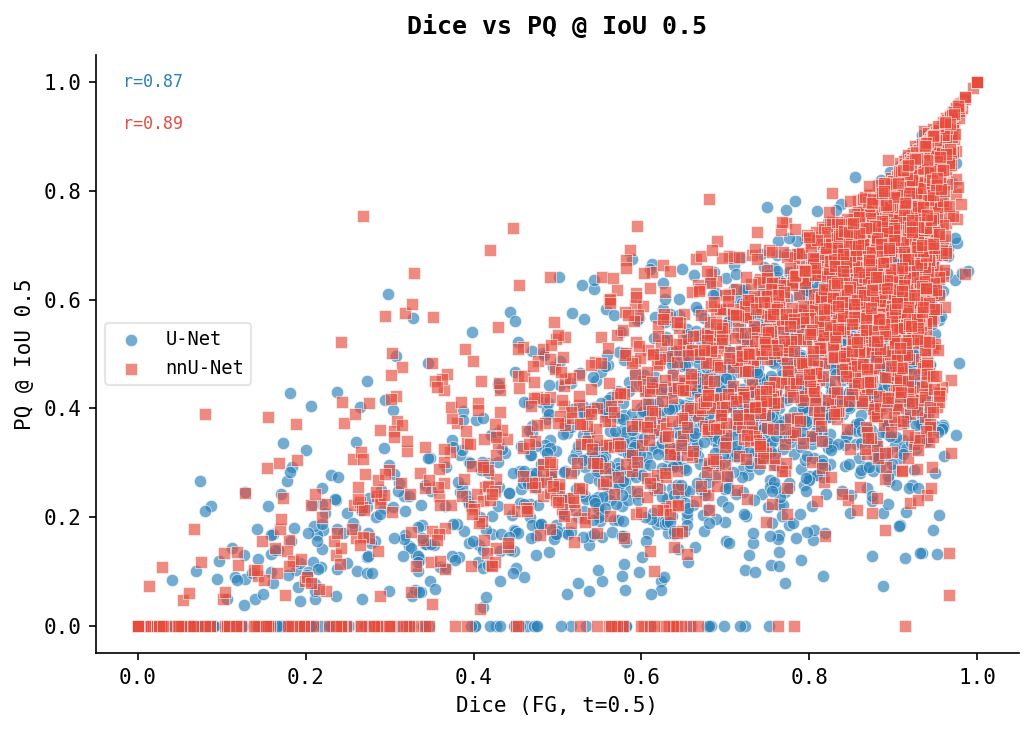
\includegraphics[width=0.85\textwidth]{../figures/scatter/scatter_dice_vs_pq_iou50.png}
\caption{Supplementary Dice--PQ scatter over the test set. Similar
  Dice values can still correspond to meaningfully different object-level
  quality.}
\label{fig:appendix-dice-vs-pq}
\end{figure}

\section{Additional Qualitative Examples}

\subsection{Additional Test Comparisons}

\begin{figure}[H]
\centering
\begin{subfigure}[t]{0.98\textwidth}
  \centering
  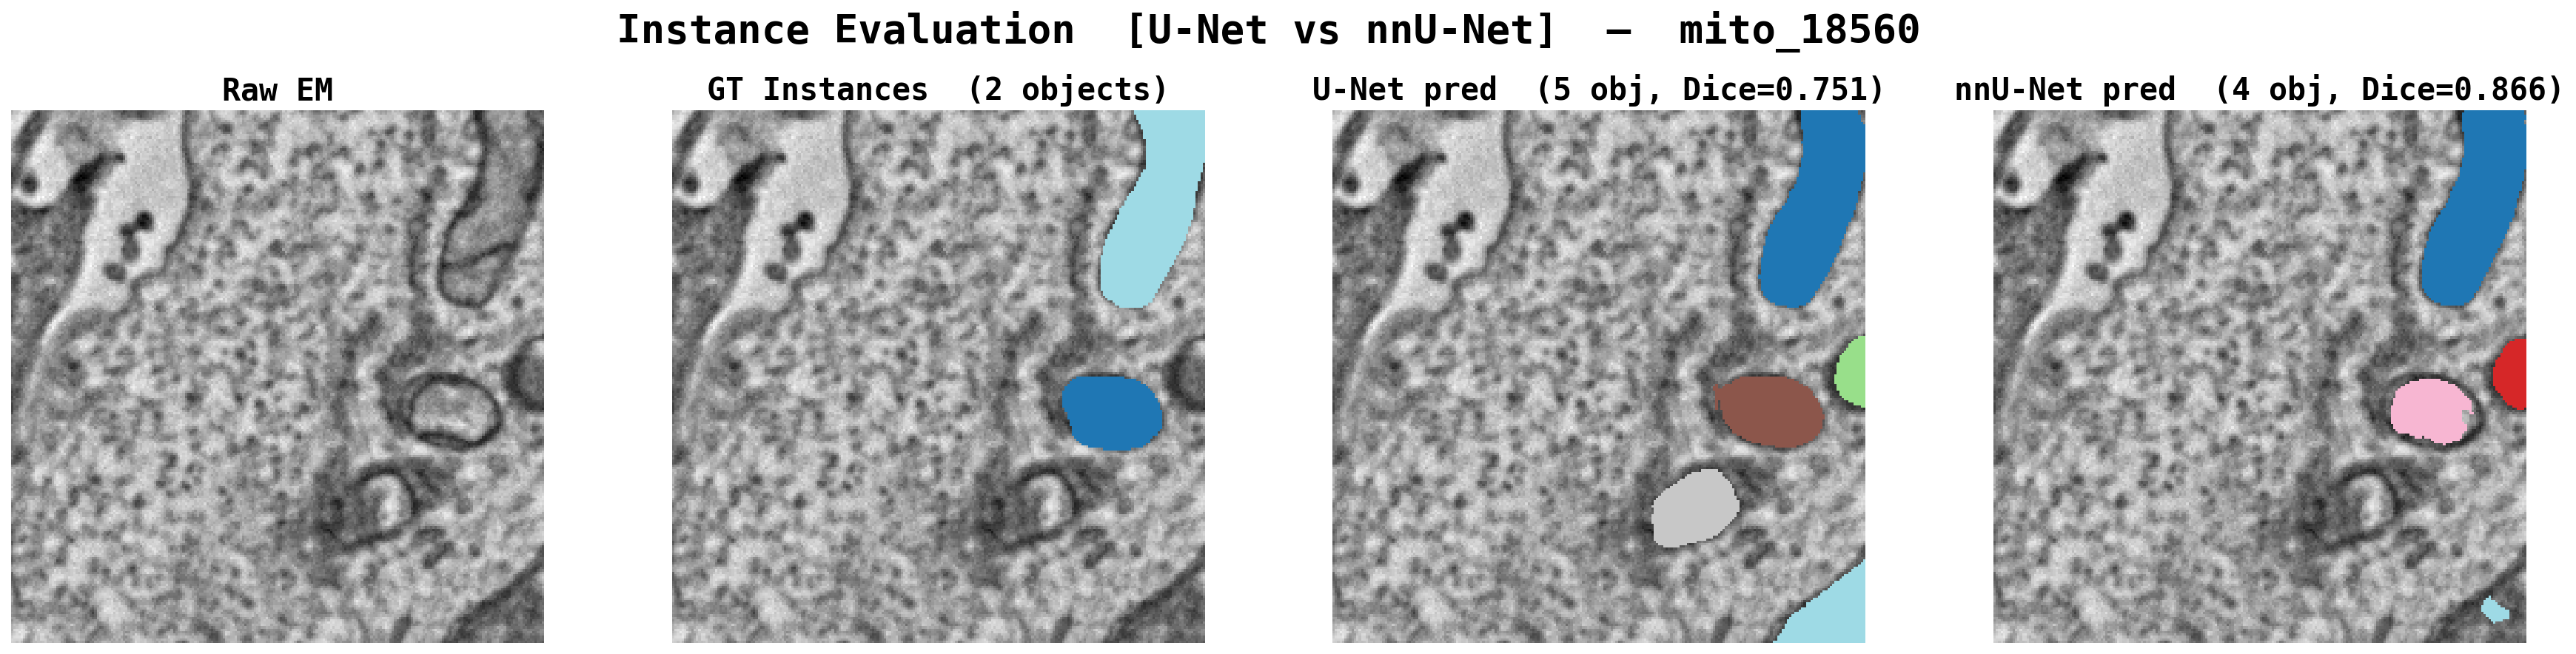
\includegraphics[width=\linewidth]{../figures/eval_instances/mito_18560_unet_vs_nnunet_instances.png}
  \caption{\texttt{mito\_18560}: additional test comparison example.}
\end{subfigure}
\vspace{0.8em}
\begin{subfigure}[t]{0.98\textwidth}
  \centering
  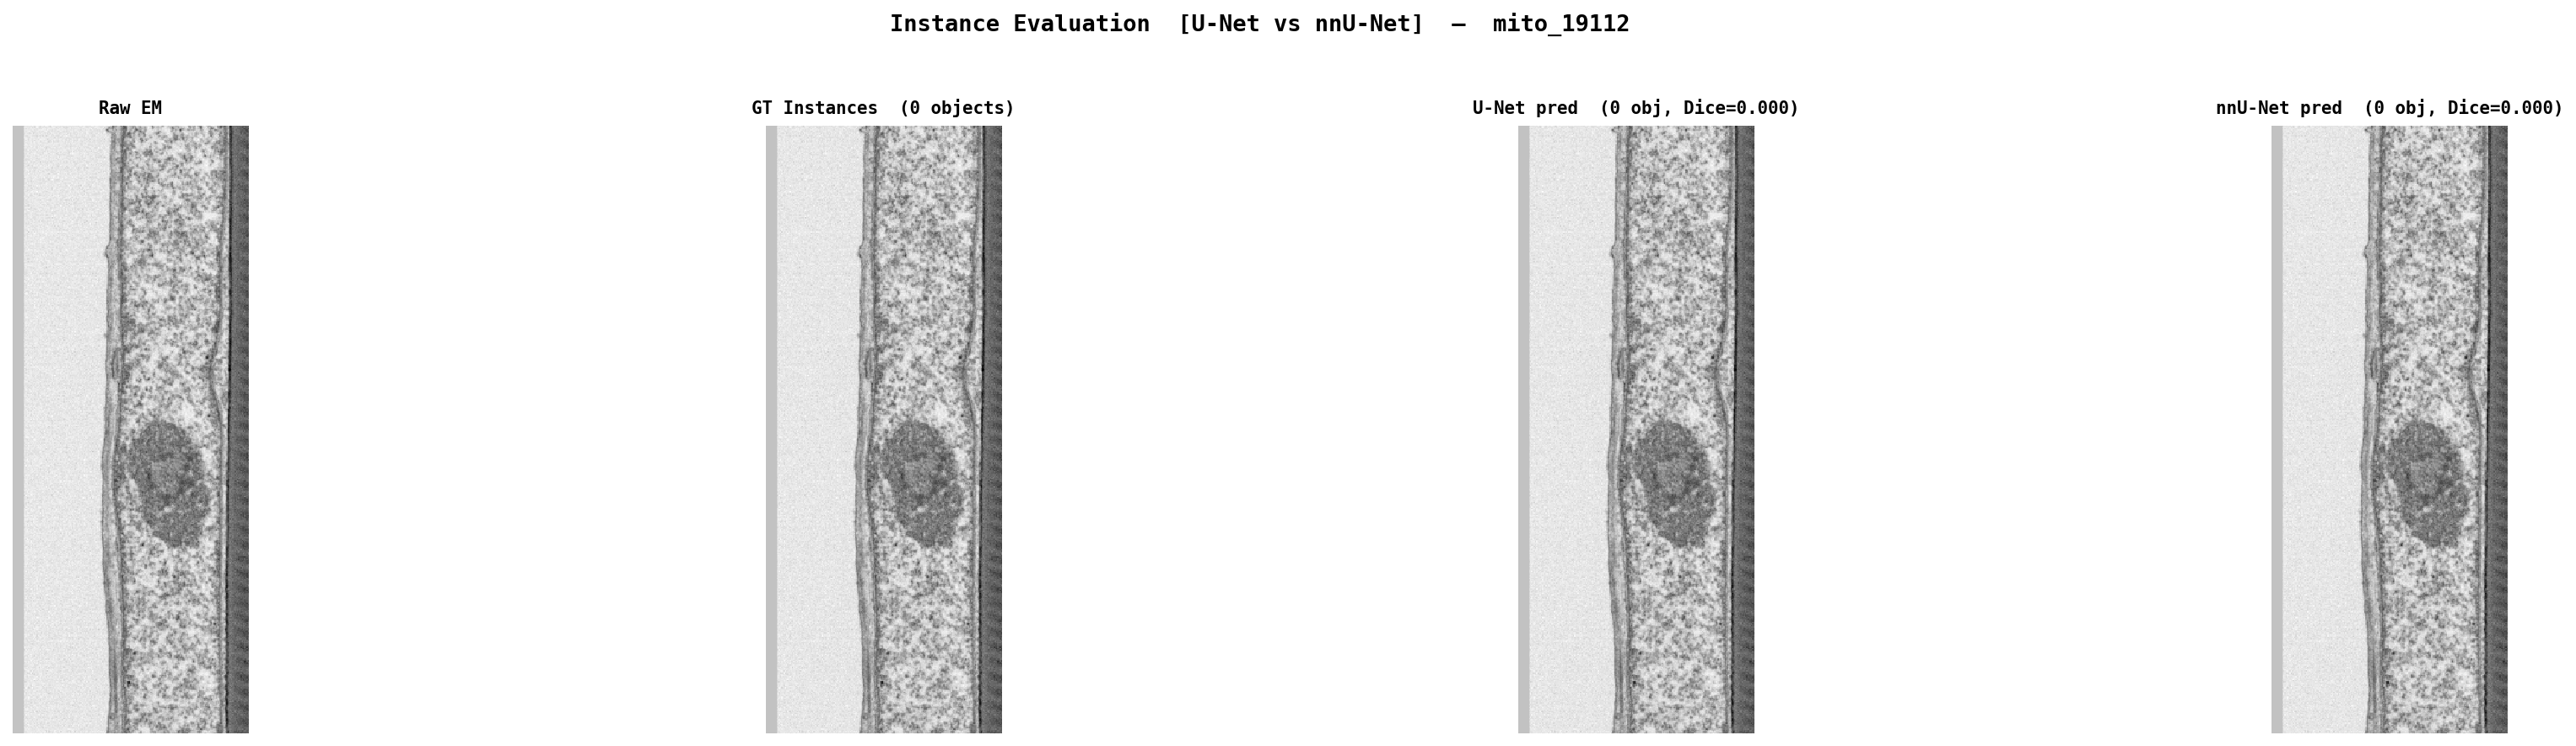
\includegraphics[width=\linewidth]{../figures/eval_instances/mito_19112_unet_vs_nnunet_instances.png}
  \caption{\texttt{mito\_19112}: additional test comparison example.}
\end{subfigure}
\caption{Additional qualitative comparisons between U-Net and nnU-Net on the test set.}
\label{fig:appendix-qualitative-1}
\end{figure}

\begin{figure}[H]
\centering
\begin{subfigure}[t]{0.98\textwidth}
  \centering
  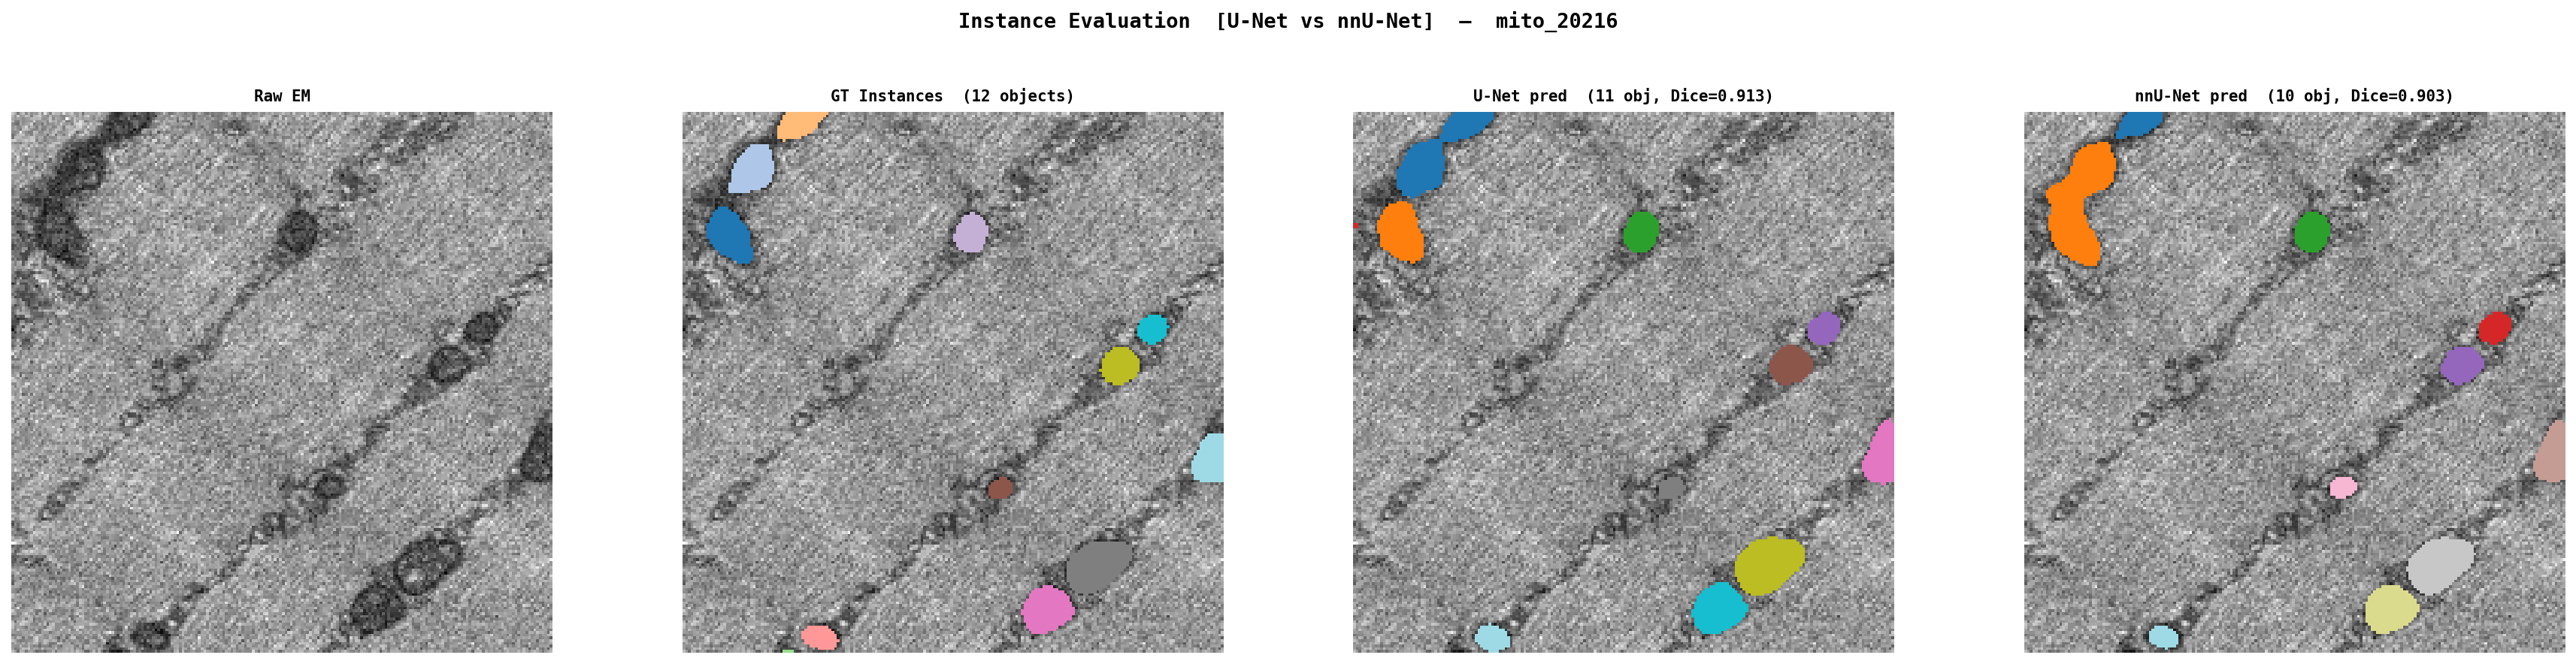
\includegraphics[width=\linewidth]{../figures/eval_instances/mito_20216_unet_vs_nnunet_instances.png}
  \caption{\texttt{mito\_20216}: additional test comparison example.}
\end{subfigure}
\vspace{0.8em}
\begin{subfigure}[t]{0.98\textwidth}
  \centering
  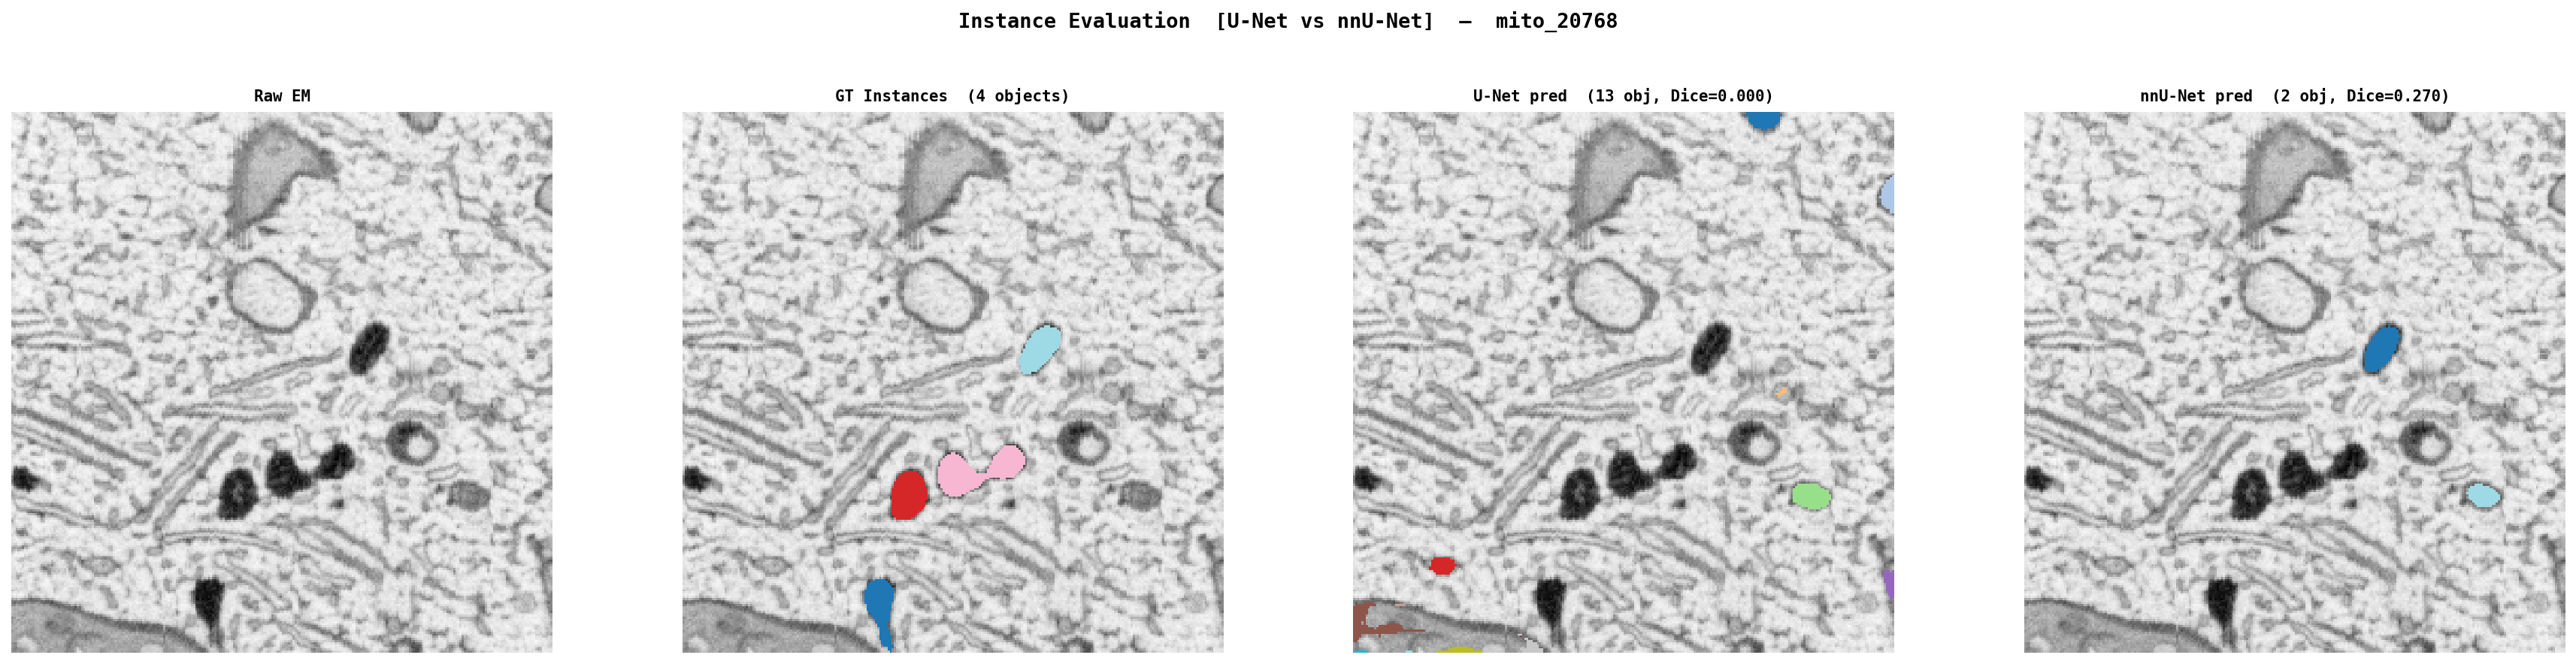
\includegraphics[width=\linewidth]{../figures/eval_instances/mito_20768_unet_vs_nnunet_instances.png}
  \caption{\texttt{mito\_20768}: additional test comparison example.}
\end{subfigure}
\caption{Further qualitative comparisons between U-Net and nnU-Net on difficult
  test slices.}
\label{fig:appendix-qualitative-2}
\end{figure}

\subsection{Additional Corner Cases}

\begin{figure}[H]
\centering
\begin{subfigure}[t]{0.86\textwidth}
  \centering
  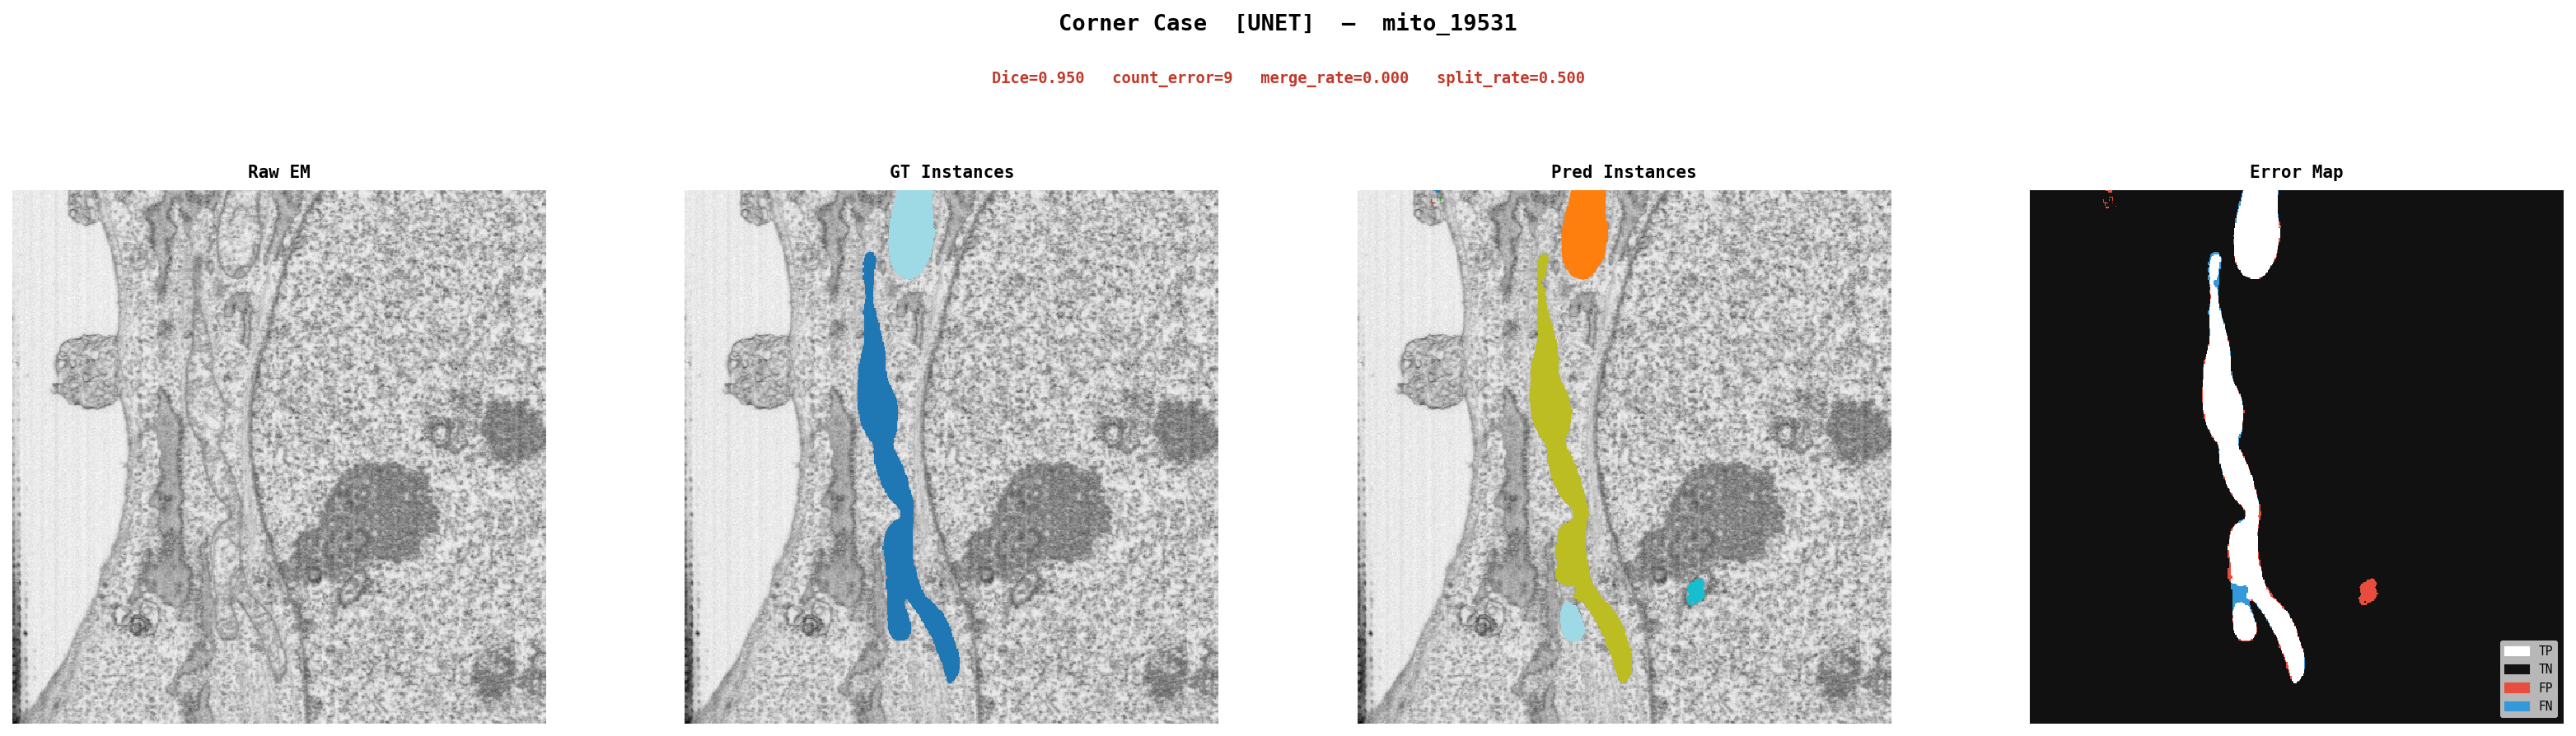
\includegraphics[width=\linewidth]{../figures/corner_cases/unet_mito_19531_corner_final.png}
  \caption{\texttt{mito\_19531}: additional U-Net corner case.}
\end{subfigure}
\vspace{0.8em}
\begin{subfigure}[t]{0.86\textwidth}
  \centering
  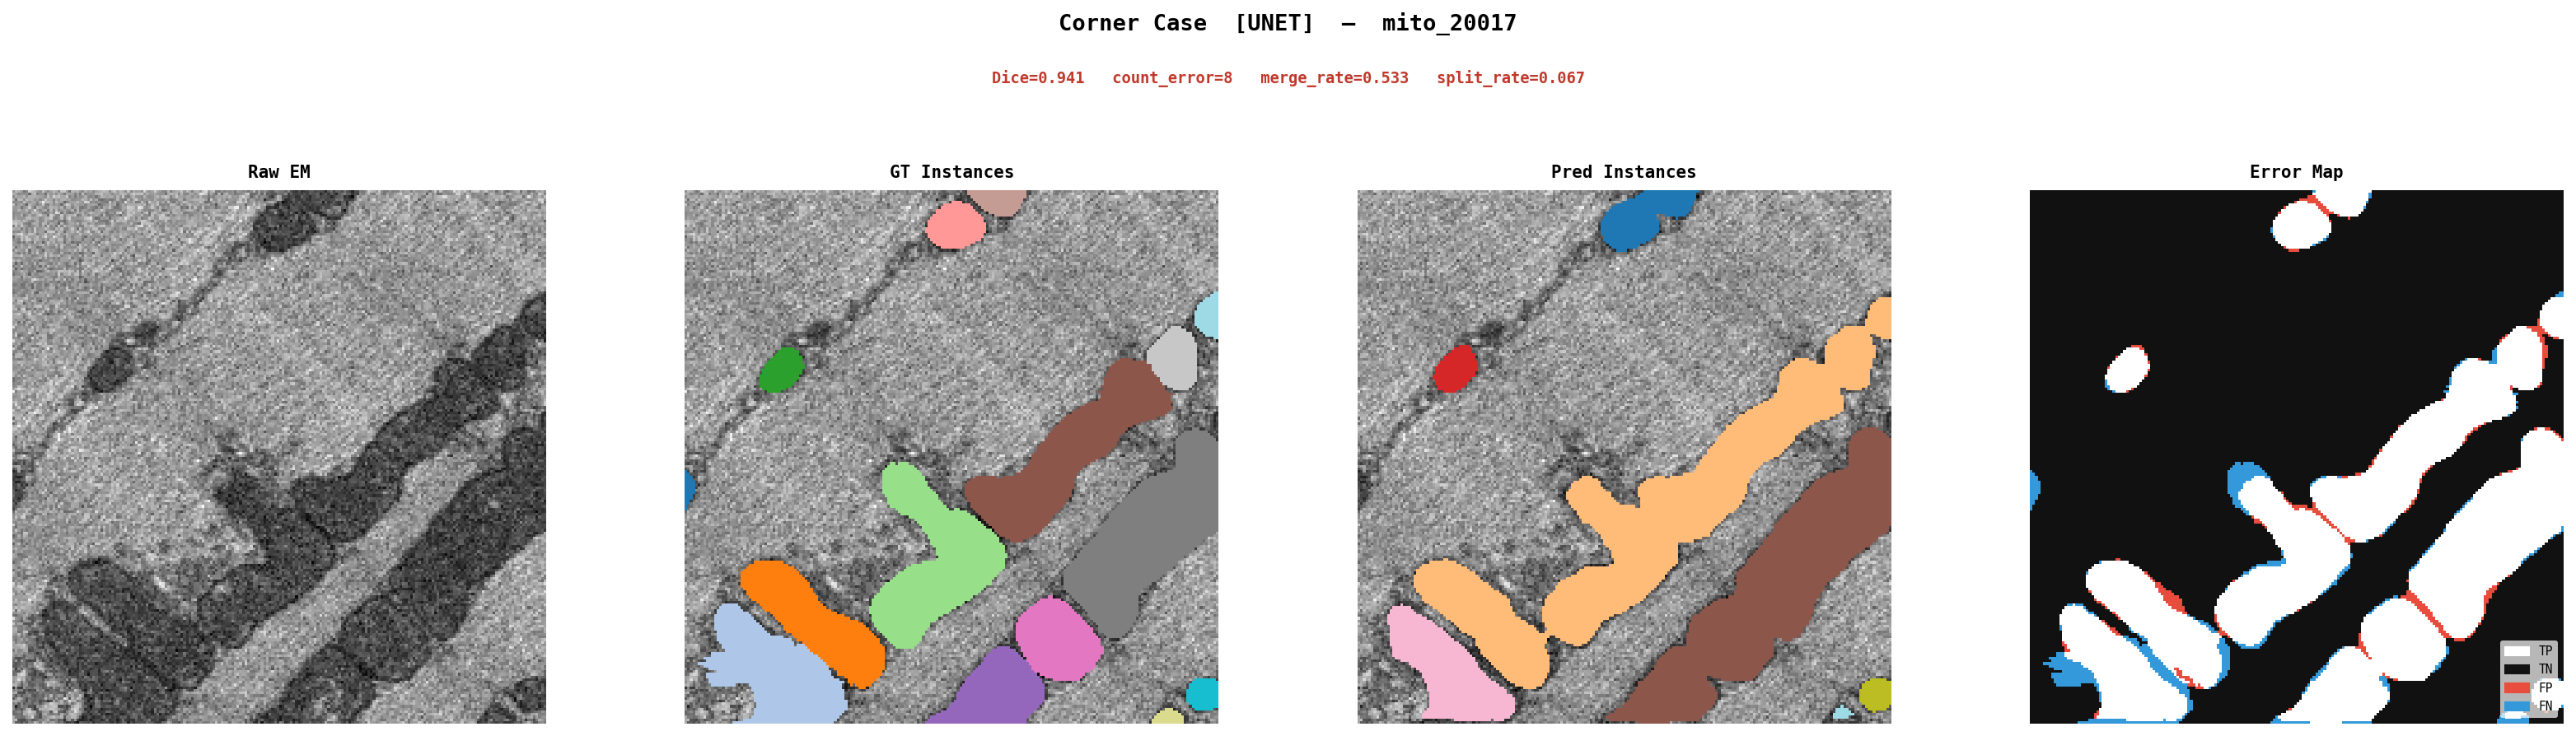
\includegraphics[width=\linewidth]{../figures/corner_cases/unet_mito_20017_corner_final.png}
  \caption{\texttt{mito\_20017}: additional U-Net corner case.}
\end{subfigure}
\caption{Additional U-Net corner cases.}
\label{fig:appendix-unet-corners}
\end{figure}

\begin{figure}[H]
\centering
\begin{subfigure}[t]{0.86\textwidth}
  \centering
  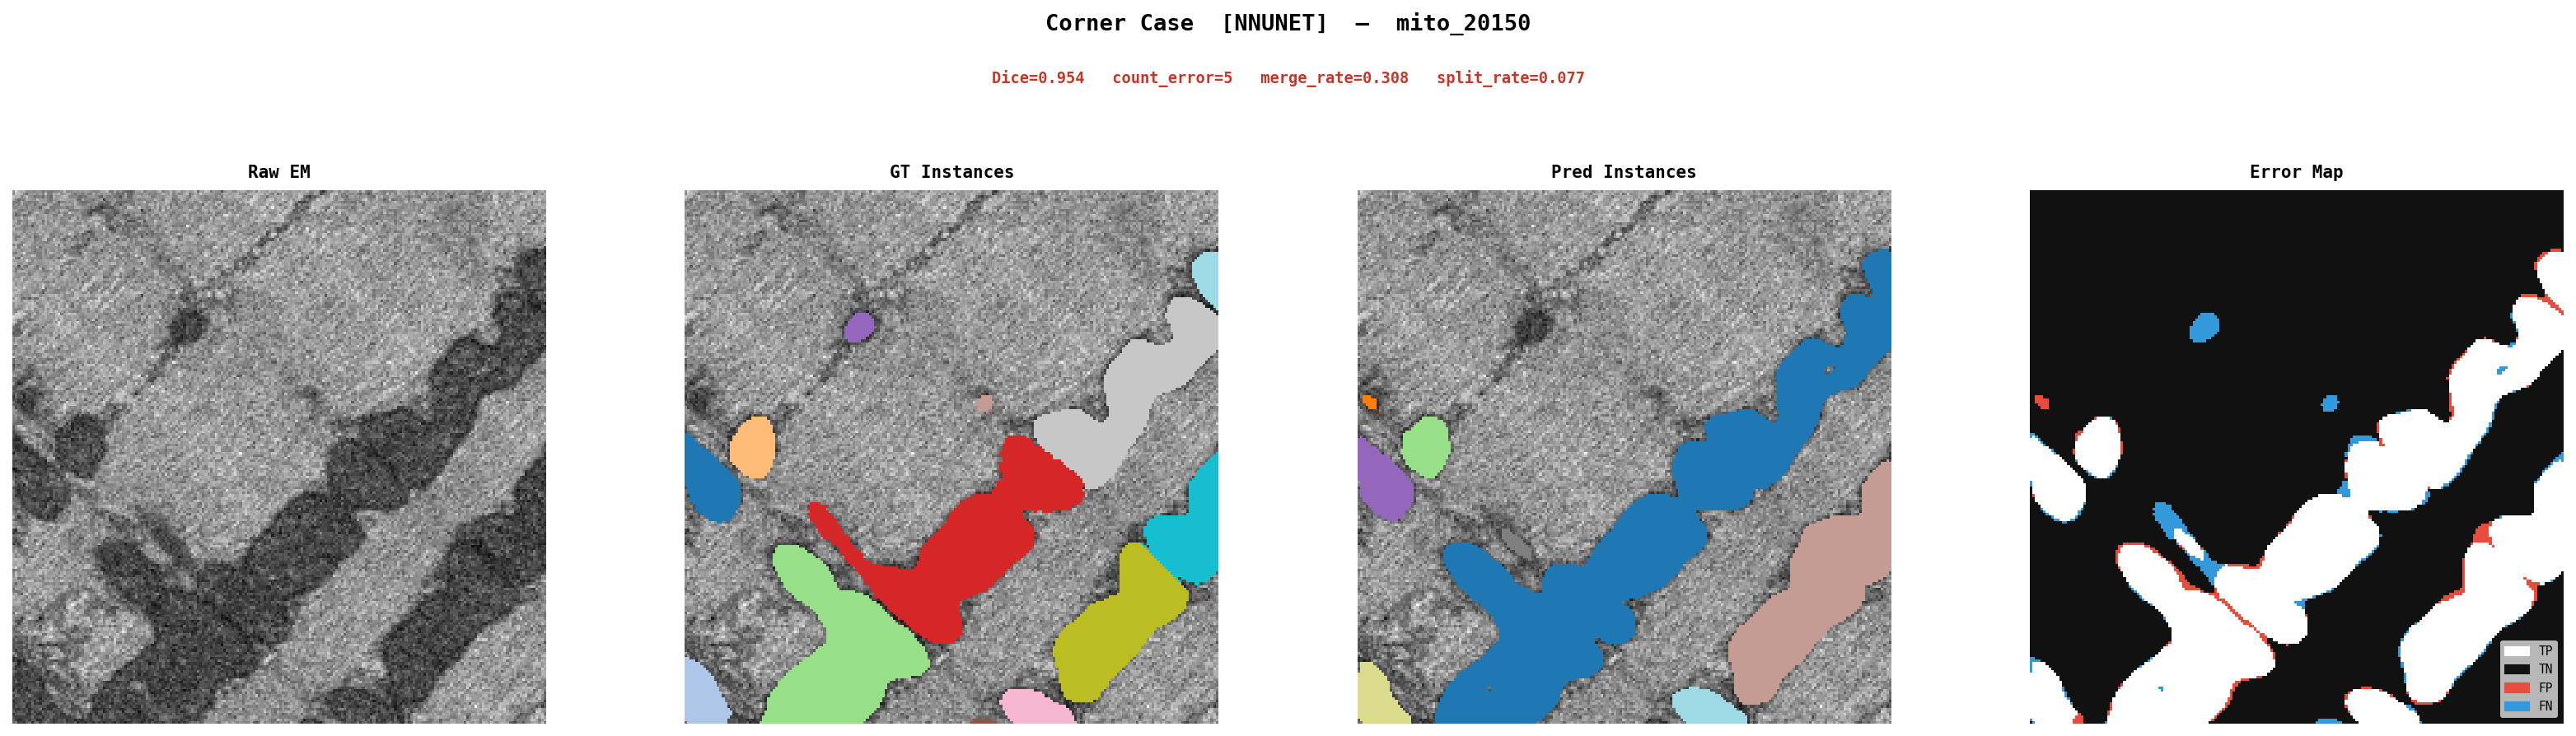
\includegraphics[width=\linewidth]{../figures/corner_cases/nnunet_mito_20150_corner_final.png}
  \caption{\texttt{mito\_20150}: additional nnU-Net corner case.}
\end{subfigure}
\vspace{0.8em}
\begin{subfigure}[t]{0.86\textwidth}
  \centering
  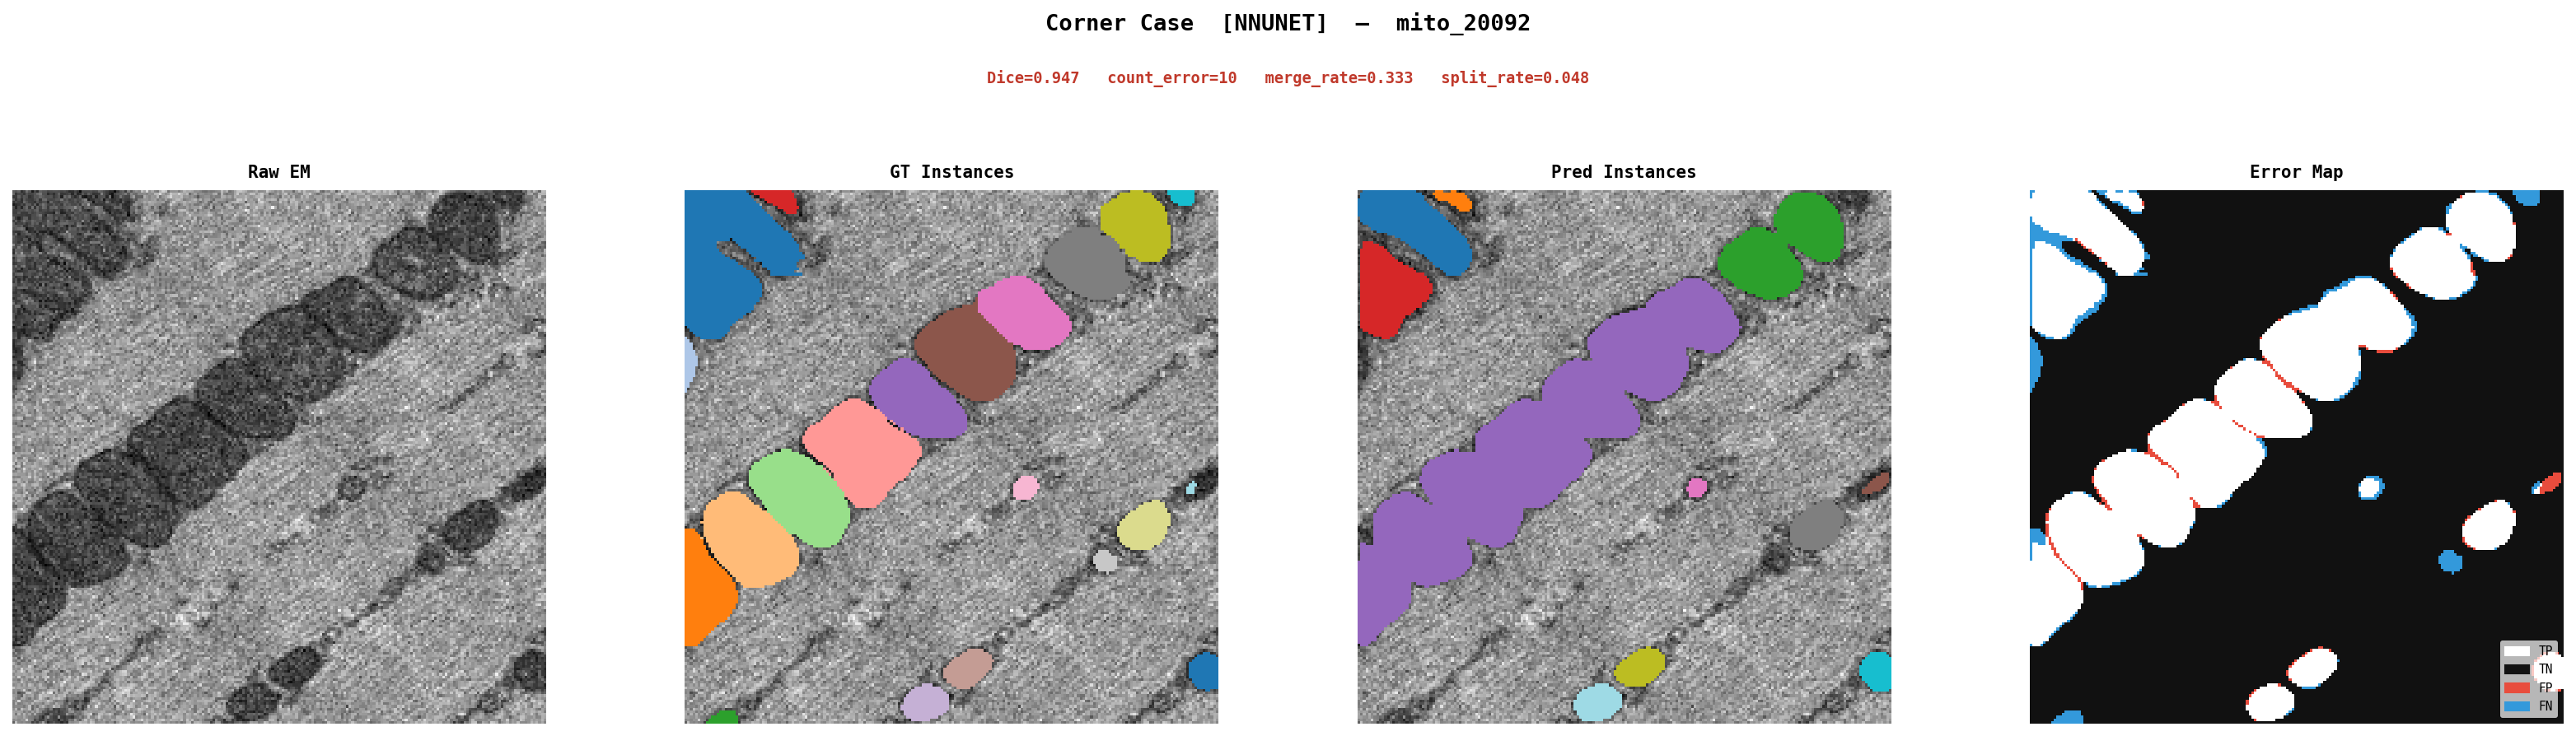
\includegraphics[width=\linewidth]{../figures/corner_cases/nnunet_mito_20092_corner_final.png}
  \caption{\texttt{mito\_20092}: additional nnU-Net corner case.}
\end{subfigure}
\caption{Additional nnU-Net corner cases.}
\label{fig:appendix-nnunet-corners}
\end{figure}

\end{document}
